%*******************************************************************************
%****************************** Fifth Chapter *********************************
%*******************************************************************************

\chapter{Quantifying Human-Humanoid Imitation Activities} \label{chapter7}
%
%% **************************** Define Graphics Path **************************
%\ifpdf
%    \graphicspath{{chapter7/figs/raster/}{chapter7/figs/PDF/}{chapter7/figs/}}
%\else
%    \graphicspath{{chapter7/figs/vector/}{chapter7/figs/}}
%\fi
\graphicspath{{figs/chapter7/PDF/}}


%
%%**************************** %Broad Purpose  **********************************
%\section*{Summary and broad purpose of the chapter}
%* How long (number of words)?
%* Deadline
%* What have you got?
%


\section{Human-Humanoid Imitation Experiment} % \label{sec:experiment}
We conducted an experiment in the context of human-humanoid imitation (HHI) activities 
where participants were asked to imitate repetitions of simple horizontal 
and vertical arm movements performed by NAO, a humanoid robot from Aldebaran \cite{gouaillier2009}.
Such simple movements were repeated ten times for the participant as the 
robot performed those arm movements in a face-to-face imitation activity.
Additionally, wearable inertial measurement unit (IMU) sensors were attached 
to the right hand of the participant and to the left hand of the robot (Figure~\ref{fig:hri} A,C).
Data was then collected at a sampling rate of 50Hz with four NeMEMSi IMU sensors
which provide tri-axial data of the accelerometer, gyroscope and magnetometer sensors and
quaternions \cite{Comotti2014}. 
A further description of the NeMEMSi IMU sensors is given in Appendix \ref{appendix:b}.
%%---------------------------------(FIGURE)-------------------------------------
\begin{figure}
  \centering
  \includegraphics[width=1.0\textwidth]{hri}
    \caption{
	{\bf Human-humanoid imitation activities.} 
		Face-to-face human-humanoid imitation (HHI) activities for 
		(A) HHI of horizontal arm movement, 
		(B) Humanoid horizontal arm movement,
		(C) HHI of vertical arm movement, and 
		(D) Humanoid vertical arm movement.
        }
    \label{fig:hri}
\end{figure}
%%---------------------------------(FIGURE)------------------------------------

\subsection{Experiment of HHI activities}
In the human-humanoid imitation (HHI) experiment four neMEMSi sensors \cite{Comotti2014} were used 
in which two sensors were attached to the right hand of the participant 
and two sensors were attached to the left hand of the humanoid robot.
Then, each participant was asked to imitate repetitions of simple horizontal
and vertical arm movements performed by the humanoid robot in the following conditions:
(i) ten repetitions of horizontal arm movement at normal (HN) and faster (HF) speed (Figure~\ref{fig:hri} A), and
(ii) ten repetitions of vertical arm movement at normal (VN) and faster (VF) speed (Figure~\ref{fig:hri} C).
The normal and faster speed of arm movements is 
defined by the duration in number of samples of one repetition of NAO's arm movements.
We select NAO's arm movements duration 
to distinguish between normal and faster arm movements
as NAO's movements have less variation between repetition to repetition.
The duration for one repetition of the horizontal arm movement at normal speed, HN, 
is about 5 seconds considering that each repetition last around 250 samples.
For horizontal arm movement at faster speed, HF, each repetition were performed 
in around 2 seconds which correspond to 90 samples of data.
The vertical arm movement at normal speed, VN, were performed  in 6 seconds 
which is around 300 samples of data.
For vertical arm movement at faster speed, VF, each repetition lasts about 2.4 seconds 
which correspond to 120 samples of data.
To visualise the distinction between normal and faster speed for horizontal 
and vertical arm movements, Fig~\ref{fig:sts} shows smoothed time series 
for axes Z and Y of the gyroscope sensors with four window lengths: 
2-sec (100-samples), 5-sec (250-samples), 10-sec (500-samples) and 15-sec (750-samples).
%%---------------------------------(FIGURE)-------------------------------------
\begin{figure}[!h] 
  \centering
  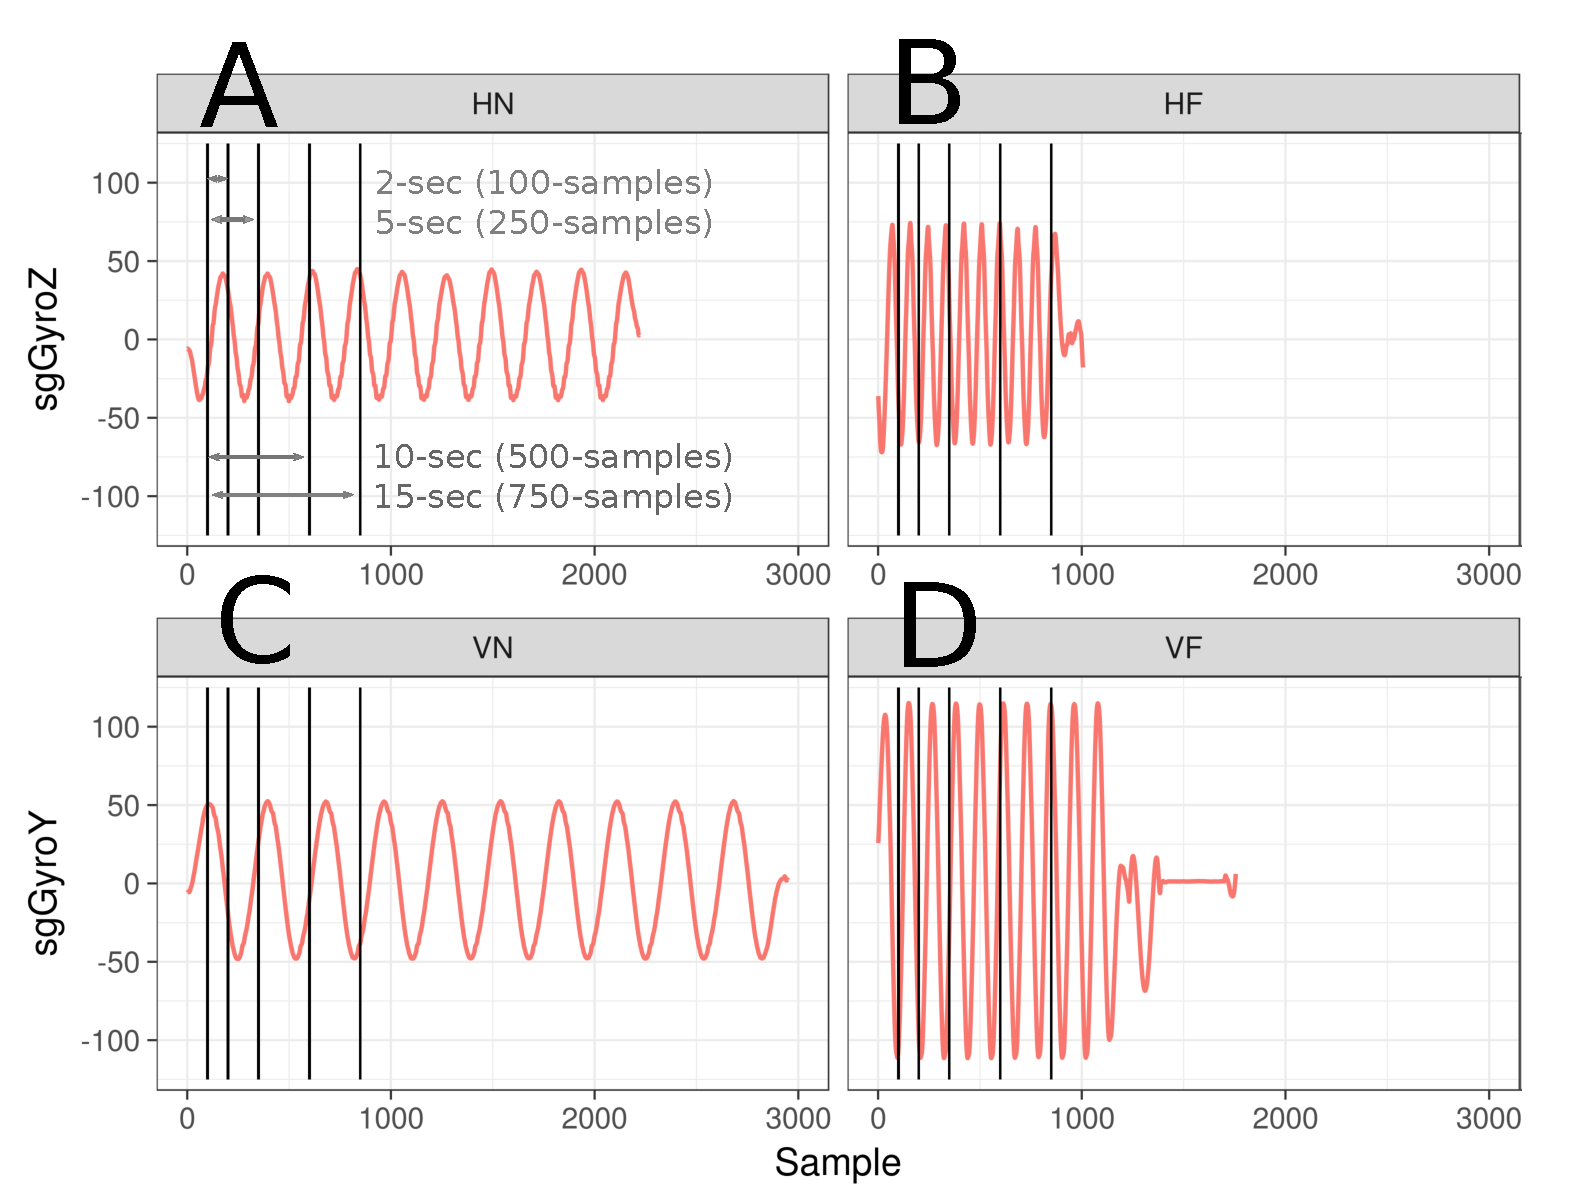
\includegraphics[width=1.0\textwidth]{sts}
    \caption{
	{\bf Time series duration of horizontal and vertical arm movements.} 
		Time series of smoothed data from gyroscope sensor 
		for different speed arm movements performed by NAO: 
		(A) Horizontal Normal arm movement, HN, 
		(B) Horizontal Faster arm movement, HF,
		(C) Vertical Normal arm movement, VN, and 
		(D) Vertical Faster arm movement, VF.
		Additionally, (A) shows window sizes for 2-seconds (100 samples), 
		5-seconds (250 samples), 10-seconds (500 samples) and 15-seconds (750 samples)
		which are also presented in (B), (C) and (D).
		R code to reproduce figure is available \cite{hwum2018}.
        }
	\label{fig:sts}
\end{figure}
%%---------------------------------(FIGURE)------------------------------------

\subsection{Time-series from Inertial Measurement Units} \label{sec:experiment:subsec:imu}


%%%%%%%%%%%%%%%%%%%%%%%%%%%%%%%%%%%%%%%%%%%%%%%%%%%%%%%%%%%%%%%%%%%%%%%%%%%%%%%%
%%%%%%%%%%%%%%%%%%%%%%%%%%%%%%%%%%%%%%%%%%%%%%%%%%%%%%%%%%%%%%%%%%%%%%%%%%%%%%%
\subsubsection{Raw data}
Considering the work of \cite{shoaib2016} which provided evidence 
of an improvement in recognition activities when combining data 
from accelerometer and gyroscope.
We focus our analysis from data of the accelerometer and gyroscope
of the NeMEMsi sensors \cite{Comotti2014} and leave the data of 
the magnetometer and quaternions for further investigation 
because of their possible variations with regard to magnetic disturbances.

Data from the accelerometer is defined by triaxial time series $A_x(n)$, $A_y(n)$, $A_z(n)$
which forms the matrix $ \boldsymbol{A}$ (Eq.~\ref{eq:A}), and the same for data from the gyroscope 
which is defined by triaxial time-series of $G_x(n)$, $G_y(n)$, $G_z(n)$ representing 
the matrix $\boldsymbol{G}$ (Eq.~\ref{eq:G}).
Both triaxial time series of each sensor, $a$ and $g$, are denoted with its respective axes 
subscripts $x,y,z$, where $n$ is the sample index  and $N$ is the same maximum length 
of all axes for the time series.
Matrices  $\boldsymbol{A}$ and $\boldsymbol{G}$ are represented as follow
%%---------------------------------(EQUATION)-------------------------------------
\begin{equation}\label{eq:A}
\boldsymbol{A} =
\begin{pmatrix}
  A_x(n) \\
  A_y(n) \\
  A_z(n)
\end{pmatrix}
=
\begin{pmatrix}
 a_x(1),a_x(2),\dots,a_x(N) \\
 a_y(1),a_y(2),\dots,a_y(N) \\
 a_z(1),a_z(2),\dots,a_z(N) 
\end{pmatrix},
\end{equation}
%%---------------------------------(EQUATION)-------------------------------------
%%---------------------------------(EQUATION)-------------------------------------
\begin{equation}\label{eq:G}
\boldsymbol{G} =
\begin{pmatrix}
 G_x(n) \\
 G_y(n) \\
 G_z(n)
\end{pmatrix}
=
\begin{pmatrix}
 g_x(1),g_x(2),\dots,g_x(N) \\
 g_y(1),g_y(2),\dots,g_y(N) \\
 g_z(1),g_z(2),\dots,g_z(N) 
\end{pmatrix},
\end{equation}
%%---------------------------------(EQUATION)-------------------------------------
where $n$ is the sample index  and $N$ is the same maximum length of all axes for the time series.


%%%%%%%%%%%%%%%%%%%%%%%%%%%%%%%%%%%%%%%%%%%%%%%%%%%%%%%%%%%%%%%%%%%%%%%%%%%%%%%
%%%%%%%%%%%%%%%%%%%%%%%%%%%%%%%%%%%%%%%%%%%%%%%%%%%%%%%%%%%%%%%%%%%%%%%%%%%%%%%
%%%%%%%%%%%%%%%%%%%%%%%%%%%%%%%%%%%%%%%%%%%%%%%%%%%%%%%%%%%%%%%%%%%%%%%%%%%%%%%
\subsection{Postprocessing data}
After the collection of raw data from four NeMEMsi sensors,
time synchronisation alignment and interpolation were performed 
in order to create time series with the same length and synchronised time.
We refer the reader to Appendix~\ref{appendix:b} for technical information 
about the time synchronisation process and IMU sensors.



%%%%%%%%%%%%%%%%%%%%%%%%%%%%%%%%%%%%%%%%%%%%%%%%%%%%%%%%%%%%%%%%%%%%%%%%%%%%%%%
\subsubsection{Data normalization}

Data is normalised to have zero mean and unit variance 
using sample mean and sample standard deviation \cite{loffe2015}.
The sample mean and sample standard deviation using $x(n)$ is given by
%%---------------------------------(EQUATION)-------------------------------------
\begin{equation}\label{eq:ms}
\mu_{x(n)}= \frac{1}{N} ( \sum_{i=1}^N x(i) ), \quad  \sigma_{x(n)} =  \sqrt{ \frac{  \sum_{1=1}^N ( x(i) - \mu_{x(n)} )^2 }{ N-1 }  },      
\end{equation}
%%---------------------------------(EQUATION)-------------------------------------
then the normalised data, $\hat{x}(n)$, is computed as follows
%%---------------------------------(EQUATION)-------------------------------------
\begin{equation}\label{eq:normalization}
\hat{x} (n) = \frac{   x(n) -  \mu_{x(n)}  }{   \sigma_{x(n)} }.   
\end{equation}
%%---------------------------------(EQUATION)-------------------------------------



%%%%%%%%%%%%%%%%%%%%%%%%%%%%%%%%%%%%%%%%%%%%%%%%%%%%%%%%%%%%%%%%%%%%%%%%%%%%%%%
\subsubsection{Smothing data}
Using a low-pass filter is the common way to either capture
the low frequencies that represent \%99 of the human body energy 
or to get the  gravitational  and body motion components of accelerations \cite{anguita2013}.
However, for this work the main focus in on the conservation of 
the structure of the time series in terms of the width and heights where, 
for instance, Savitzky-Golay filter can help to accomplish such task \cite{press1992}.
Savitzky-Golay filter is based on the principle of moving window avere  
which preserves the area under the curve (the zeroth moment)
and its mean position in time (the first moment) 
but the line width (the second moment) is violated 
and that results, for example, in the case of spectrometric data
where a narrow spectral line is presented with reduced height  
and width. 
The aim of Savitzky-Golay filtering is to find the filter 
coefficients $c_n$ that preserve higher momentums
which are based on local least-square polynomial approximations 
\cite{savitzkygolay1964, press1992, schafer2011}.
Hence, Savitzky-Golay coefficients are therefore computed using an R function 
\texttt{sgolay(p,n,m)} where \texttt{p} is the filter order, 
\texttt{n} is the filter length (must be odd) 
and \texttt{m} is the $m$-th derivative of the filter coefficients  \cite{Rsignal}.
Smoothed signal is represented with a tilde over the original signal: $\tilde{x}(n)$.



%%%%%%%%%%%%%%%%%%%%%%%%%%%%%%%%%%%%%%%%%%%%%%%%%%%%%%%%%%%%%%%%%%%%%%%%%%%%%%%
\subsubsection{Window size data}
With regard to the window size, \cite{shoaib2016} investigated its effects 
using seven window lengths (2, 5, 10, 15, 20, 25, 30 seconds)
and combination of inertial sensors (accelerometer, gyroscope and linear acceleration sensor)
in activity recognition performance for repetitive activities 
(walking, jogging and biking) and less repetitive activities 
(smoking, eating, giving a talk or drinking a coffee).
Similarly, \cite{shoaib2016} experimented with 
different window size effect to conclude that the increase of window size 
improved the recognition of complex activities because these required 
a large window to learn the repetitive motion patterns.
Also, \cite{shoaib2016} concluded that the use of large window size 
improve the recognition performance of less repetitive activities which mainly 
involve random hand gestures.

For the activities in this thesis which are mainly repetitive, we selected 
only four window sizes: 2-s window (100 samples), 5-s window (250 samples), 
10-s (500 samples) and 15-s window (750 samples) (Figure~\ref{fig:sts}).




\section{Human-Humanoid Imitation Activities} %\section{Results}\label{sec:results}
We investigated the robustness and weaknesses of the reconstructed state spaces (RRSs) 
using the uniform time-delay embedding technique (UTDE) 
and recurrence plots (RPs) for recurrent quantification analysis (RQA) 
methodologies in the following conditions: 
\begin{itemize}

\item Three levels of smoothness for the normalised data (sg0zmuv, sg1zmuv and sg2zmuv), 
	computed from two different filter lengths (29 and 159) with the same polynomial degree 
	of 5 using the function \texttt{sgolay(p,n,m)} \cite{Rsignal},

\item Four velocities arm movement activities: 
	horizontal normal (HN), horizontal faster (HF), vertical normal (VN), and vertical faster (VF),
	and

\item Four window lengths: \{2-sec (100 samples), 5-sec (250 samples), 
	10-sec (500 samples) and 15-sec (750 samples) \}.

\end{itemize}





%%%%%%%%%%%%%%%%%%%%%%%%%%%%%%%%%%%%%%%%%%%%%%%%%%%%%%%%%%%%%%%%%%%%%%%%%%%%%%%
%%%%%%%%%%%%%%%%%%%%%%%%%%%%%%%%%%%%%%%%%%%%%%%%%%%%%%%%%%%%%%%%%%%%%%%%%%%%%%%
\subsection{Time series}
After the data collection in the experiment, raw time series were windowed, normalised and smoothed.
We only present 10-sec (500 samples) window length time series, due to space limitations, 
for three participants (p01, p01 and p03) performing horizontal arm movements (axis GyroZ) 
and vertical arm movements (axis GyroY) (Figs \ref{fig:tsH} and \ref{fig:tsV}).
We consider different levels of smoothness of the normalised data 
with two different Savitzky-Golay filter lengths (29 and 159) 
with the same polynomial degree of 5 using \texttt{sgolay(p,n,m)} \cite{Rsignal}.
 

%%---------------------------------(FIGURE)-------------------------------------
\begin{figure}[!h]
  \centering
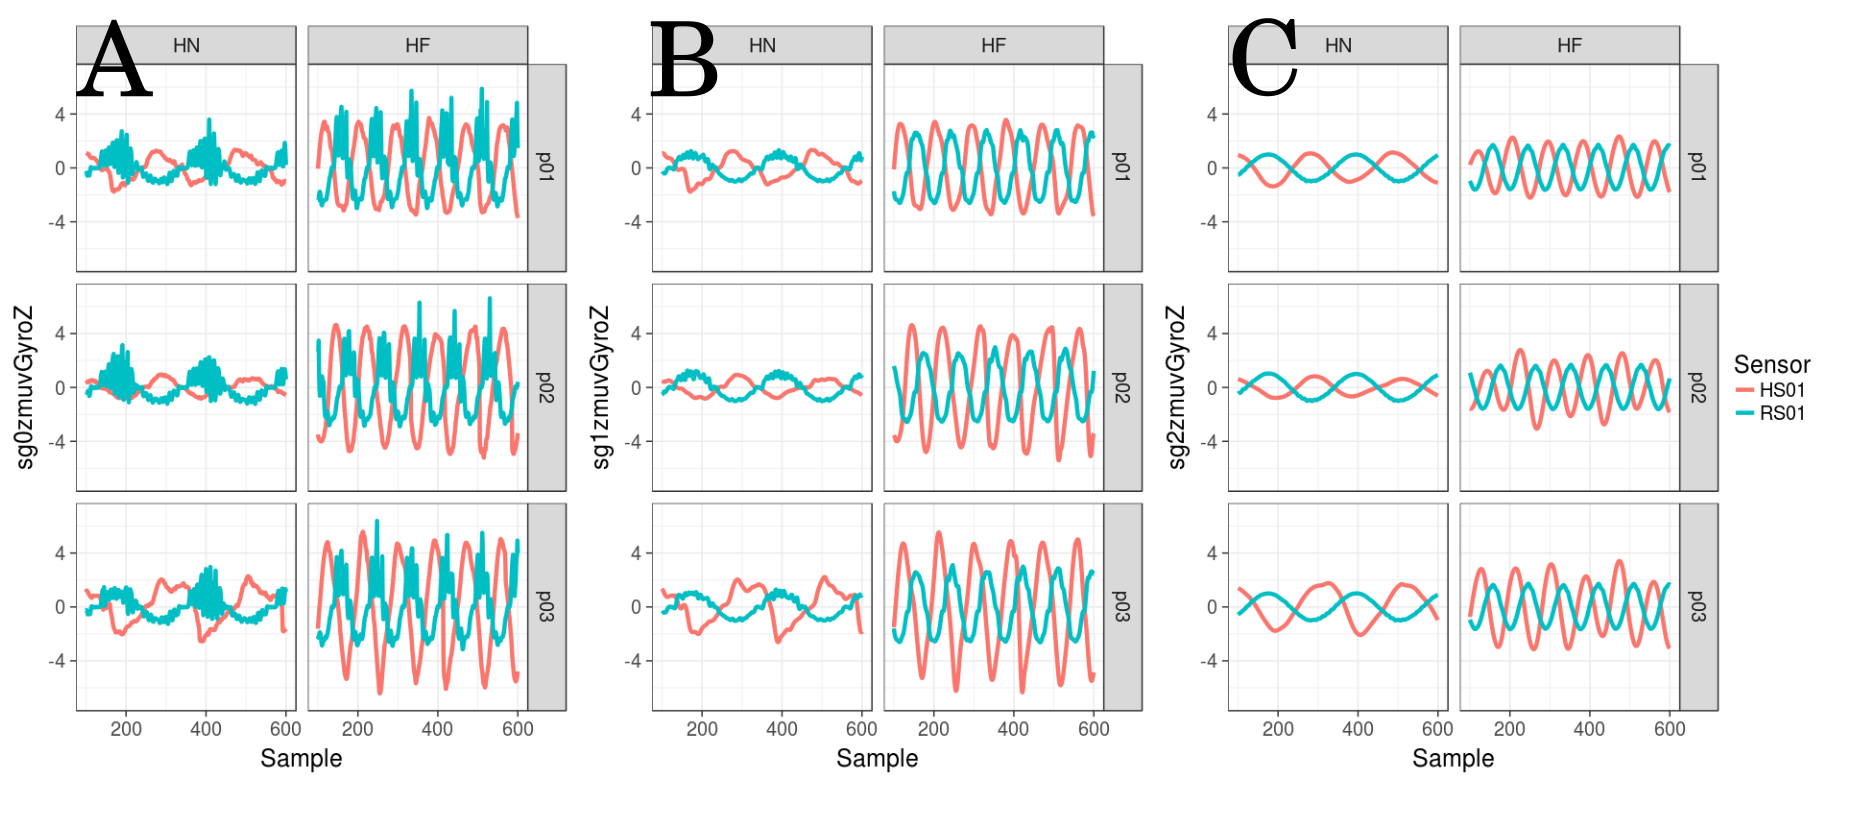
\includegraphics[width=1.0\textwidth]{tsHv03}
    	\caption{ 
	{\bf Time series for horizontal arm movements.}
		(A) raw-normalised (sg0zmuvGyroZ), 
		(B) normalised-smoothed 1 (sg1zmuvGyroZ) and
		(C) normalised-smoothed 2 (sg2zmuvGyroZ).
		Time series are only for three participants (p01, p02, and p03) 
		for horizontal movements in normal and faster velocity (HN, HF) 
		with the normalised GyroZ axis (zmuvGyroZ) 
		and with one sensor attached to the participant (HS01) 
		and other sensor attached to the robot (RS01).	
	R code to reproduce the figure is available from \cite{hwum2018}.
        }
    \label{fig:tsH}
\end{figure}
%%---------------------------------(FIGURE)------------------------------------
%%---------------------------------(FIGURE)-------------------------------------
\begin{figure}[!h]
  \centering
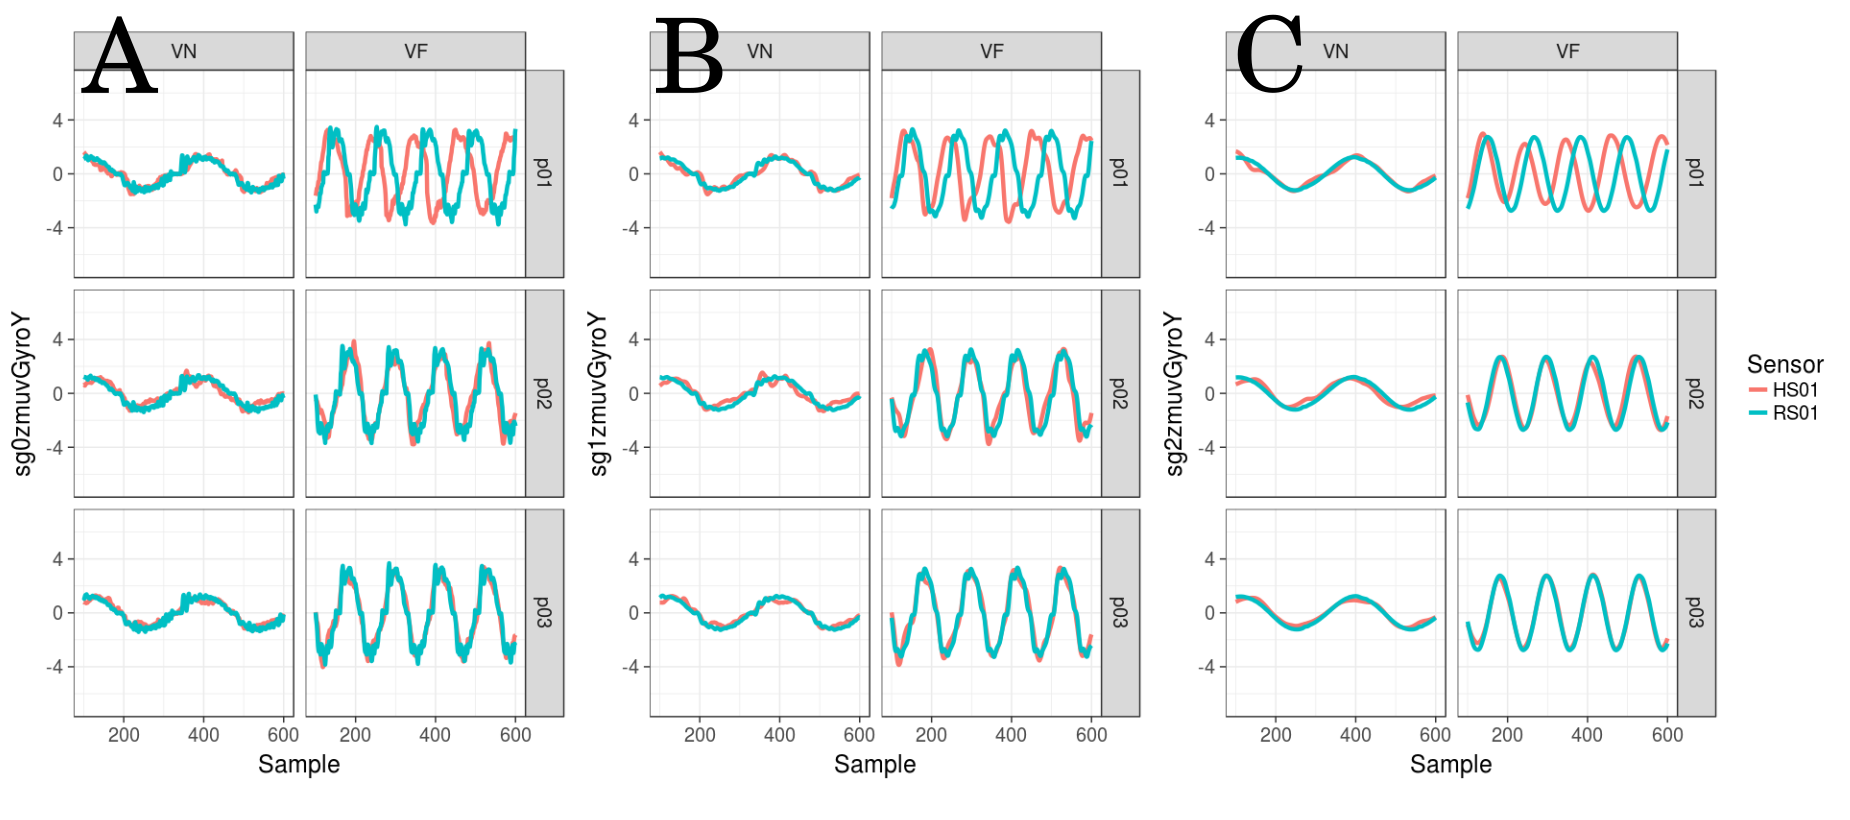
\includegraphics[width=1.0\textwidth]{tsVv03}
	\caption{ 
	{\bf Time series for vertical arm movements.}
		(A) raw-normalised (sg0zmuvGyroY), 
		(B) normalised-smoothed 1 (sg1zmuvGyroY) and
		(C) normalised-smoothed 2 (sg2zmuvGyroY).
		Time series are only for three participants (p01, p02, and p03) 
		for vertical movements in normal and faster velocity (VN, VF) 
		with the normalised GyroY axis (zmuvGyroY) 
		and with one sensor attached to the participant (HS01) 
		and other sensor attached to the robot (RS01).
		R code to reproduce the figure is available from \cite{hwum2018}.
        }
    \label{fig:tsV}
\end{figure}
%%---------------------------------(FIGURE)------------------------------------









%%%%%%%%%%%%%%%%%%%%%%%%%%%%%%%%%%%%%%%%%%%%%%%%%%%%%%%%%%%%%%%%%%%%%%%%%%%%%%%
%%%%%%%%%%%%%%%%%%%%%%%%%%%%%%%%%%%%%%%%%%%%%%%%%%%%%%%%%%%%%%%%%%%%%%%%%%%%%%%
\subsection{UTDE for time series in the context of human-robot interaction}
The first step to create reconstructed state spaces is to compute 
the minimum embedding parameters which are computed in the following section.

\subsubsection{Minimum Embedding Parameters}


Considering the time series for twenty participants,
minimum embedding dimensions were computed using False Nearest Neighbour
for horizontal and vertical arm movements. %(Figs~\ref{fig:caoH} and \ref{fig:caoV}).
Figs~\ref{fig:caoH} and \ref{fig:caoV} show that minimum embedding values appear 
to be more constant for sensor RS01 than the slightly variations of such values 
for sensor HS01.
It can also be seen that there is a minor decrease of minimum embedding values
as smoothness of time series increase. 
To have an overall minimum dimension value that represent participants,
sensors and activities, a sample mean were computed over all the minimum values 
in Figs~\ref{fig:caoH} and \ref{fig:caoV} which results in $\overline{m}_0=6$.
%%---------------------------------(FIGURE)-------------------------------------
\begin{figure}[!h]
\centering
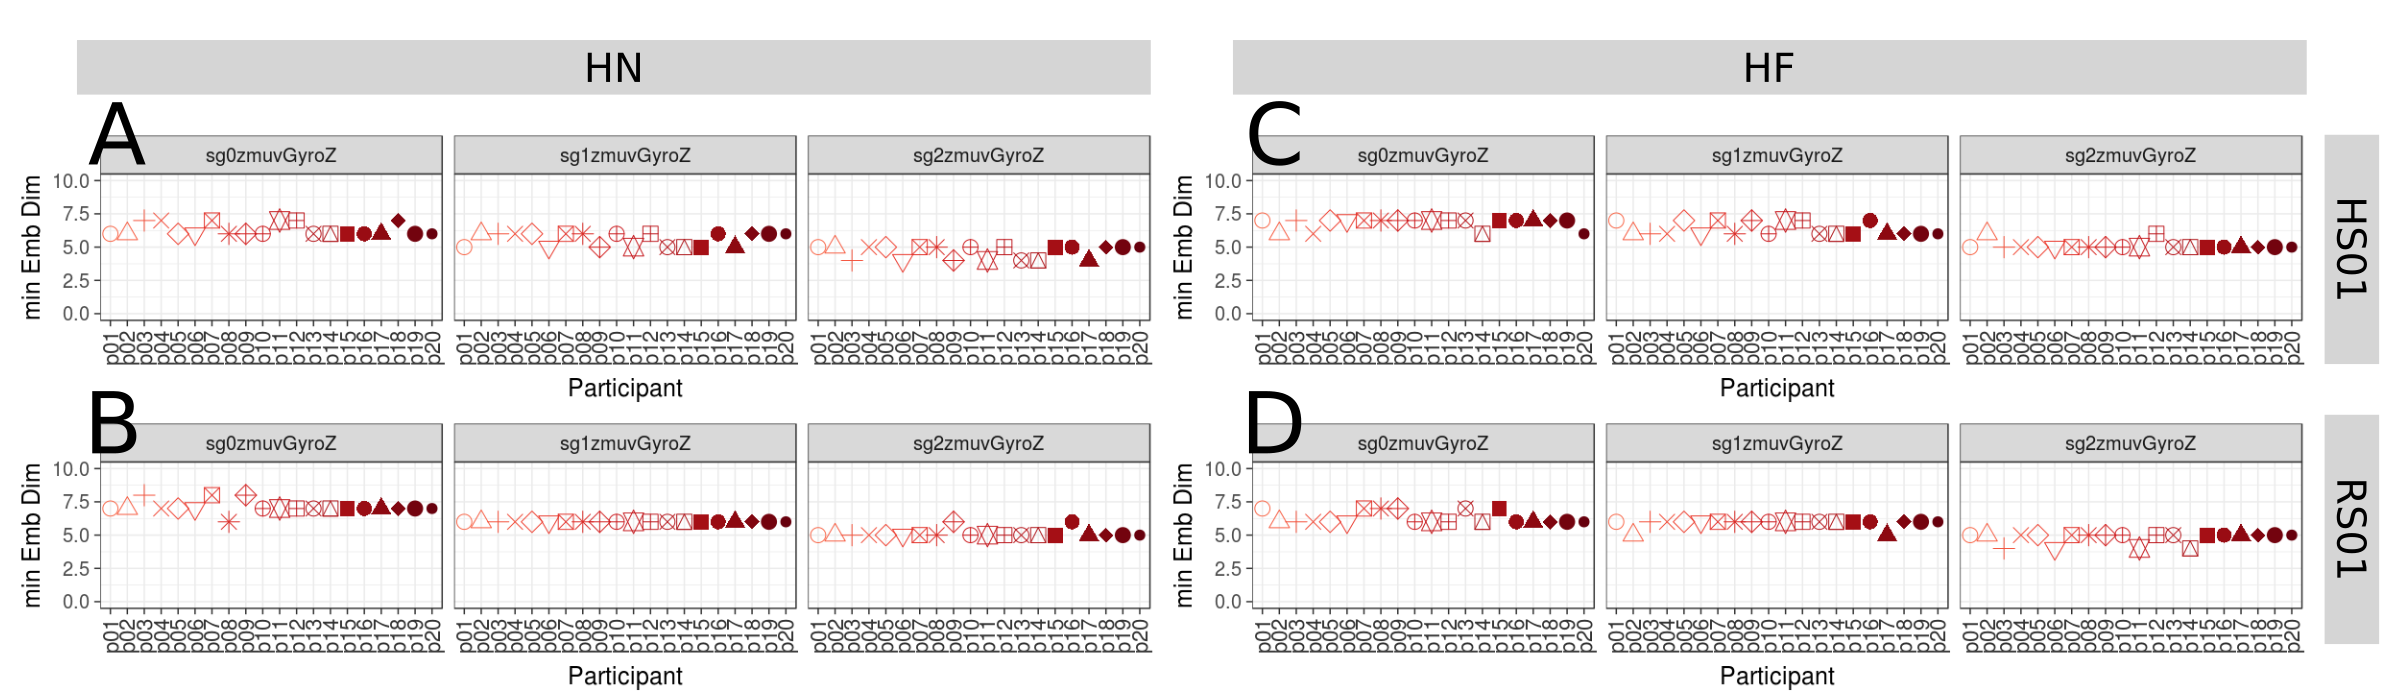
\includegraphics[width=1.0\textwidth]{cao_aHw10}
	\caption{
	{\bf Minimum embedding dimensions for horizontal arm movements.} 
		(A, B) Horizontal Normal (HN), (C, D) Horizontal Faster (HF) movements,
		(A, C) sensor attached to participants (HS01), and
		(B, D) sensor attached to robot (RS01).
		Minimum embedding dimensions are for twenty participants (p01 to p20) with
		three smoothed signals (sg0zmuvGyroZ, sg1zmuvGyroZ and sg2zmuvGyroZ)
		and window lenght of 10-sec (500 samples).
		R code to reproduce the figure is available from \cite{hwum2018}.
        }
    \label{fig:caoH}
\end{figure}
%%---------------------------------(FIGURE)------------------------------------

%%---------------------------------(FIGURE)-------------------------------------
\begin{figure}[!h]
\centering
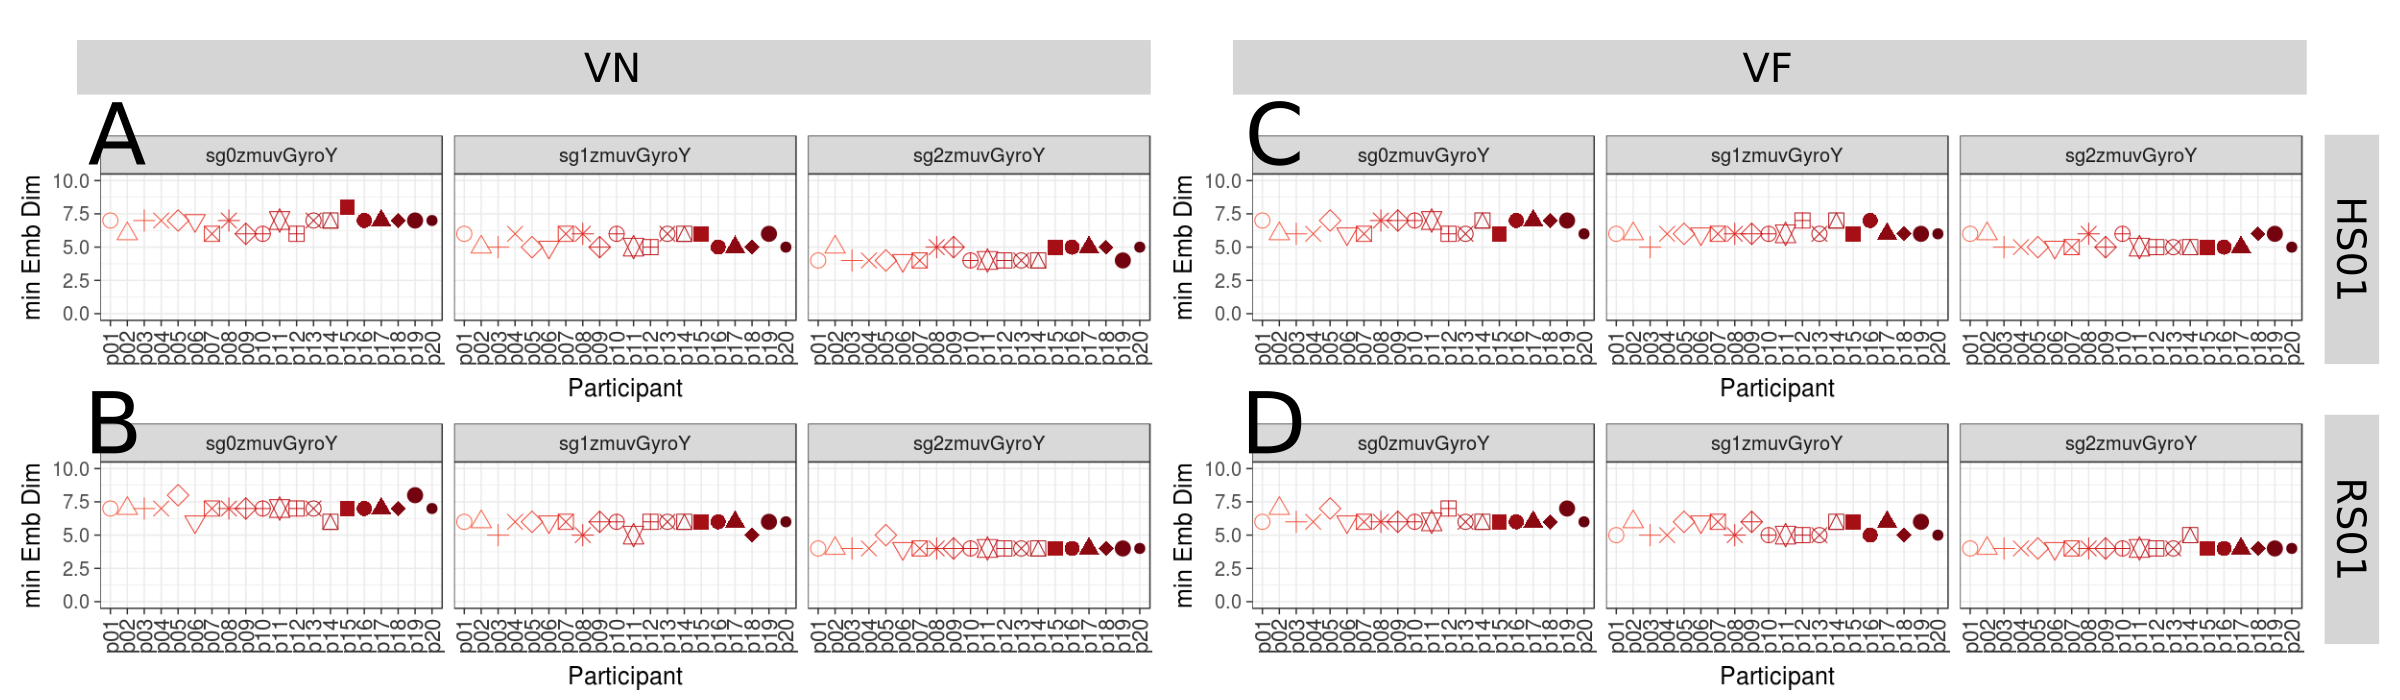
\includegraphics[width=1.0\textwidth]{cao_aVw10}
	\caption{
	{\bf Minimum embedding dimensions for vertical arm movements.} 
		(A, B) Vertical Normal (VN), (C, D) Vertical Faster (VF) movements,
		(A, C) sensor attached to participants (HS01), and		
		(B, D) sensor attached to robot (RS01).
		Minimum embedding dimensions are for twenty participants (p01 to p20) with
		three smoothed signals (sg0zmuvGyroY, sg1zmuvGyroY and sg2zmuvGyroY) 
		and window length of 10-sec (500 samples).
		R code to reproduce the figure is available from \cite{hwum2018}.
        }
    \label{fig:caoV}
\end{figure}
%%---------------------------------(FIGURE)------------------------------------



Similarly, considering the time series for twenty participants,
minimum delay values were computed as the first minimum values of the  
Average Mutual Information (AMI) for 
horizontal and vertical arm movements (Figs~\ref{fig:amiH} and \ref{fig:amiV}).

For horizontal arm movements, 
%For sensors attached to participants, 
Fig~\ref{fig:amiH}A shows that values tend to be more spread 
as the smoothness is increased which is different for Fig~\ref{fig:amiH}C
where values show no effect as the smoothness of time series increase.
In contrast, 
%for sensors attached to the robot, 
Fig~\ref{fig:amiH}B shows the values are less spread as smoothness 
is increased which we believe the reason for that is due to the high 
frequencies on robots movements in the horizontal normal movement.
However, values in Fig~\ref{fig:amiH}D tend to be spread as
smoothness is increasing which are due to very different curves in the AMI.
With regard to vertical arm movements,
values in Figs~\ref{fig:amiV}A and ~\ref{fig:amiV}C 
show an slightly increase of the spread values as the smoothness increase
and values in Fig~\ref{fig:amiV}B appear to have less variation as
the smoothness of the signals is increasing. However, 
that do not happen for the second smoothed values (sg2zmuvGyroY) in Fig~\ref{fig:amiV}D.
We also computed an overall minimum delay value that represent participants,
sensors and activities, using a sample mean of all values in 
Figs~\ref{fig:amiH} and \ref{fig:amiV} which results in $\overline{\tau}_0=8$.
%%---------------------------------(FIGURE)-------------------------------------
\begin{figure}[!h]
\centering
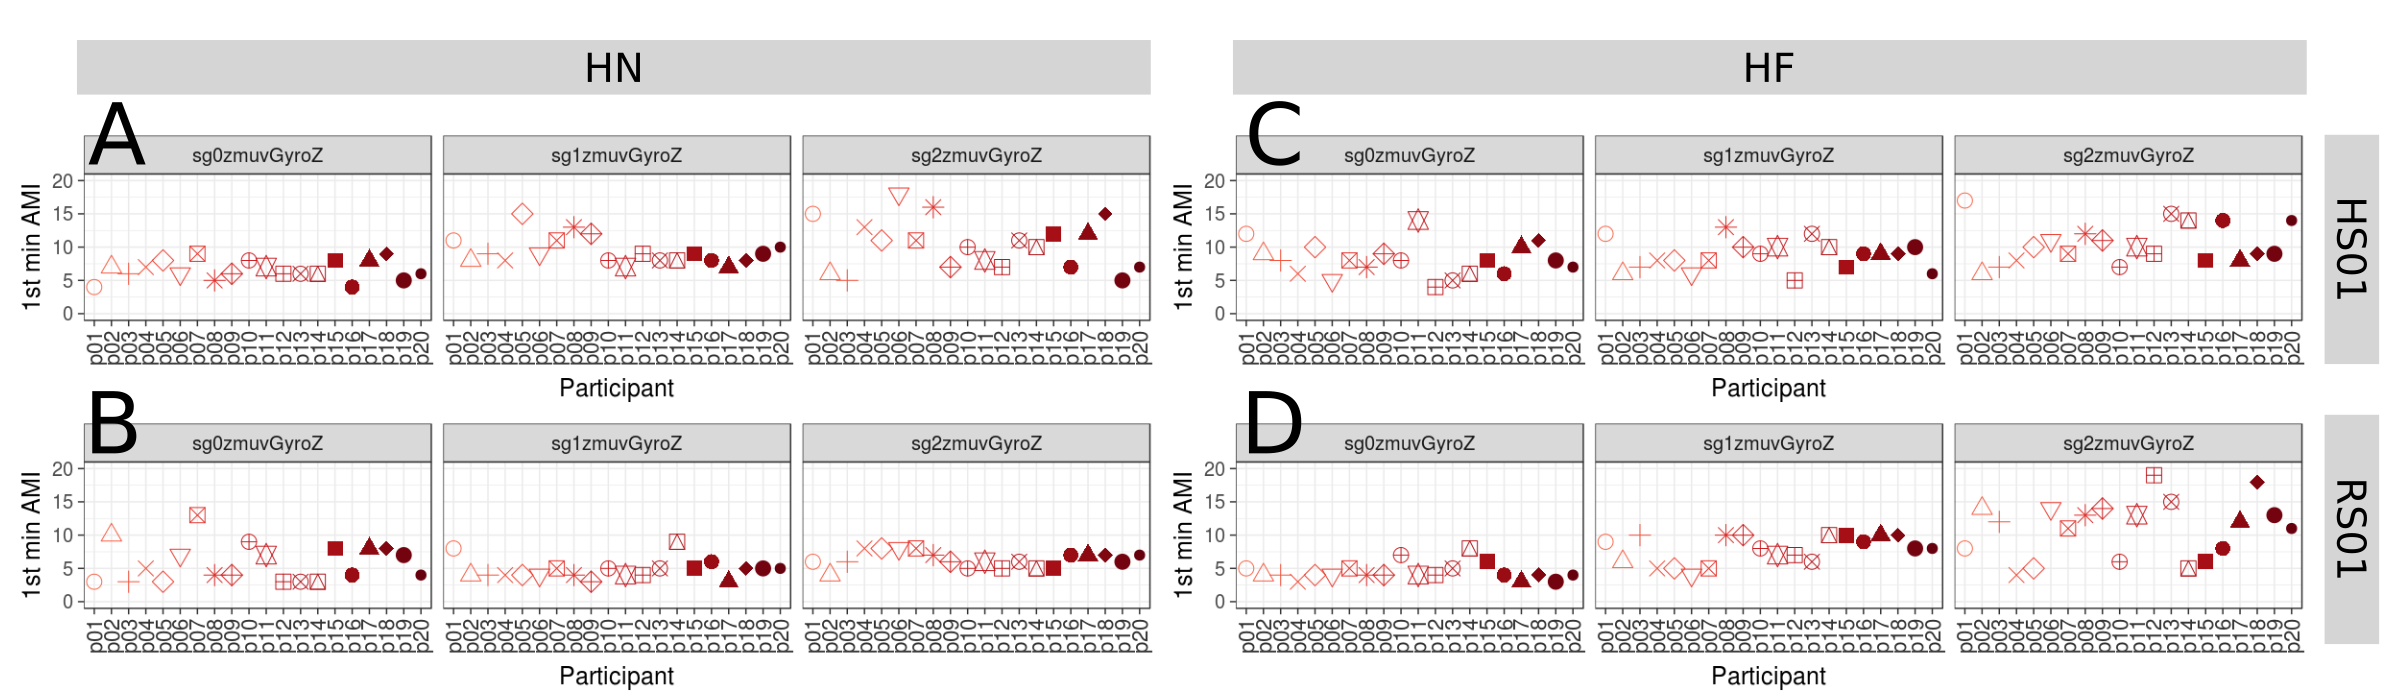
\includegraphics[width=1.0\textwidth]{ami_aHw10}
	\caption{
	{\bf First minimum AMI values for horizontal arm movements.}
		(A, B) Horizontal Normal (HN), (C, D) Horizontal Faster (HF) movements,
		(A, C) sensor attached to participants (HS01), and
		(B, D) sensor attached to robot (RS01).
		First minimum AMI values are for twenty participants (p01 to p20) 
		with three smoothed signals (sg0zmuvGyroZ, sg1zmuvGyroZ and sg2zmuvGyroZ) 
		and  window lenght of 10-sec (500 samples).
		R code to reproduce the figure is available from \cite{hwum2018}.
        }
    \label{fig:amiH}
\end{figure}
%%---------------------------------(FIGURE)------------------------------------
%%---------------------------------(FIGURE)-------------------------------------
\begin{figure}[!h]
\centering
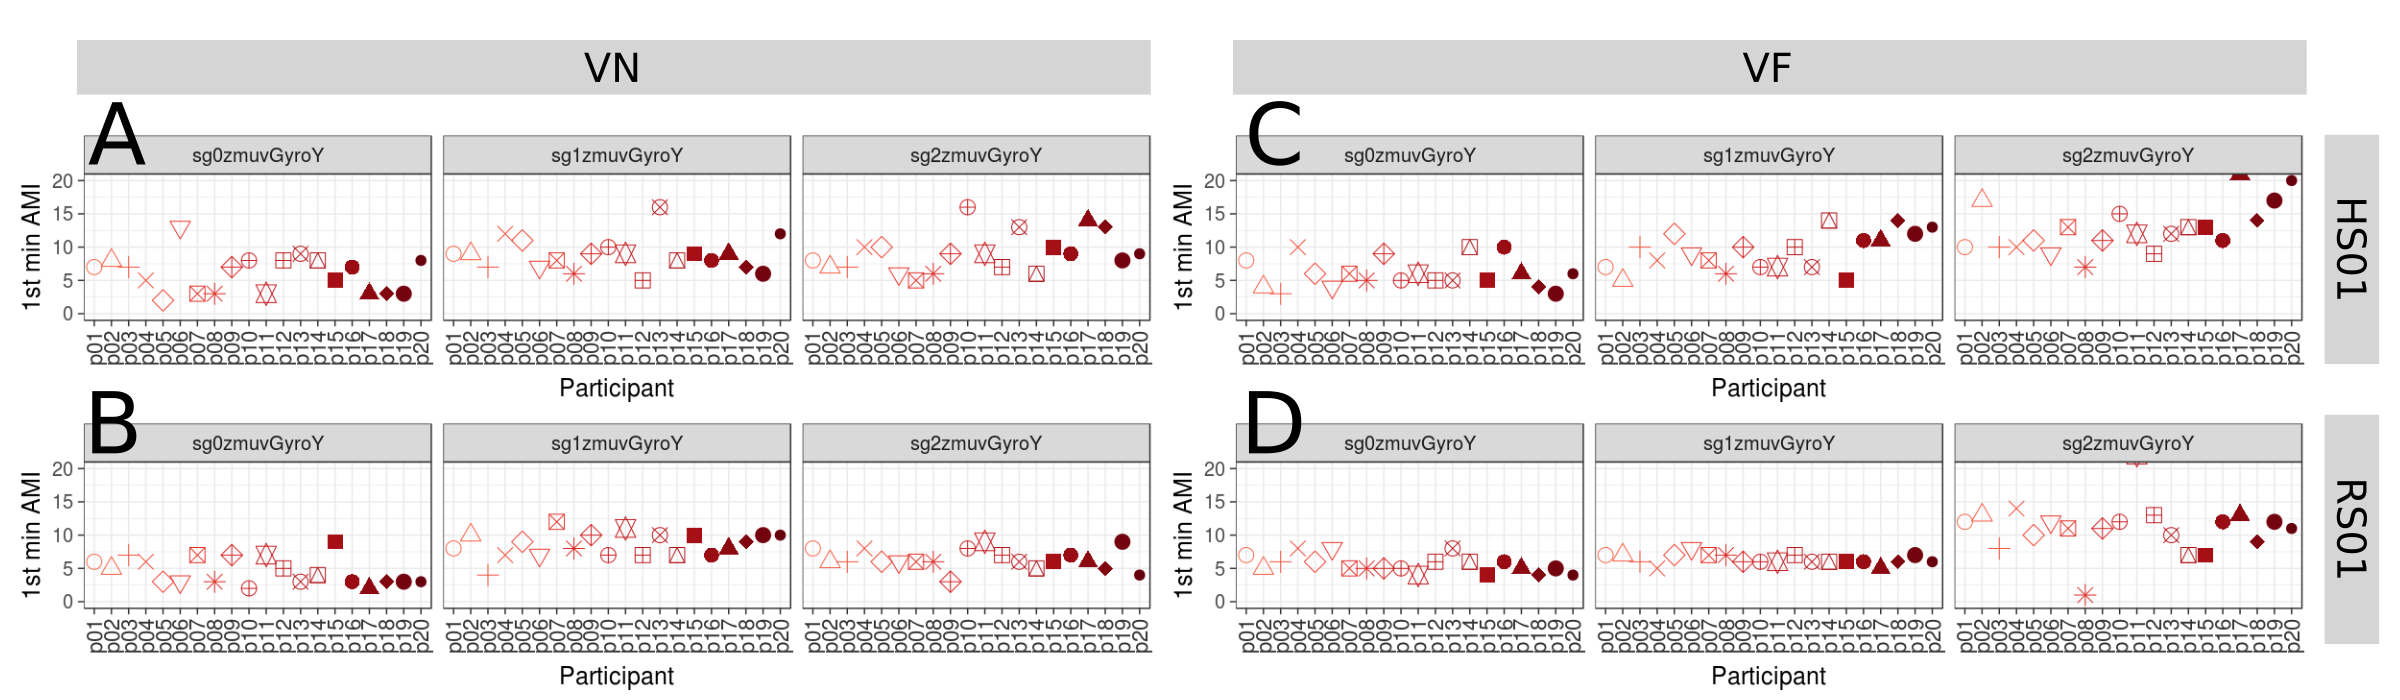
\includegraphics[width=1.0\textwidth]{ami_aVw10}
	\caption{
	{\bf First minimum AMI values for vertical arm movements.}
		(A, B) Vertical Normal (VN), (C, D) Vertical Faster (VF) movements,
		(A, C) sensor attached to participants (HS01), and
		(B, D) sensor attached to robot (RS01).
		First minimum AMI values are for twenty participants (p01 to p20) 
		with three smoothed signals (sg0zmuvGyroZ, sg1zmuvGyroZ and sg2zmuvGyroZ) 
		and  window lenght of 10-sec (500 samples).
		R code to reproduce the figure is available from \cite{hwum2018}.
        }
    \label{fig:amiV}
\end{figure}
%%---------------------------------(FIGURE)------------------------------------









\subsubsection{Reconstructed state spaces Using UTDE}
Although the implementation of Uniform Time-Delay Embedding for the 
reconstructed state space, one of the main challenges of the latter 
is the selection of embedding parameters because each time series 
is unique in terms of its structure (modulation of amplitude, frequency and phase)
\cite{ frank2010, sama2013, bradley2015}.
With that in mind, the problem is not to compute individual embedding parameters 
for each of the time series but to deal with a selecting of two parameters 
that can represent all the time series. 
Our solution for that was to compute a sample mean over all values in each of the conditions 
of the time series of Figs~\ref{fig:caoH}, \ref{fig:caoV}
for minimum dimension values and Figs~\ref{fig:amiH} and \ref{fig:amiV} for
minimum delay values, resulting in an average minimum embedding parameters 
of ($\overline{m_0}=6$, $\overline{\tau_0}=8$).
Then, the reconstructed state spaces were computed with 
($\overline{m_0}=6$, $\overline{\tau_0}=8$) and 
the first three axis of the rotated data of the PCA are shown in 
Figs~\ref{fig:rss_aHw10} for horizontal arm movements and 
Figs~\ref{fig:rss_aVw10} for vertical arm movements.
%%---------------------------------(FIGURE)-------------------------------------
\begin{figure}[!h]
\centering
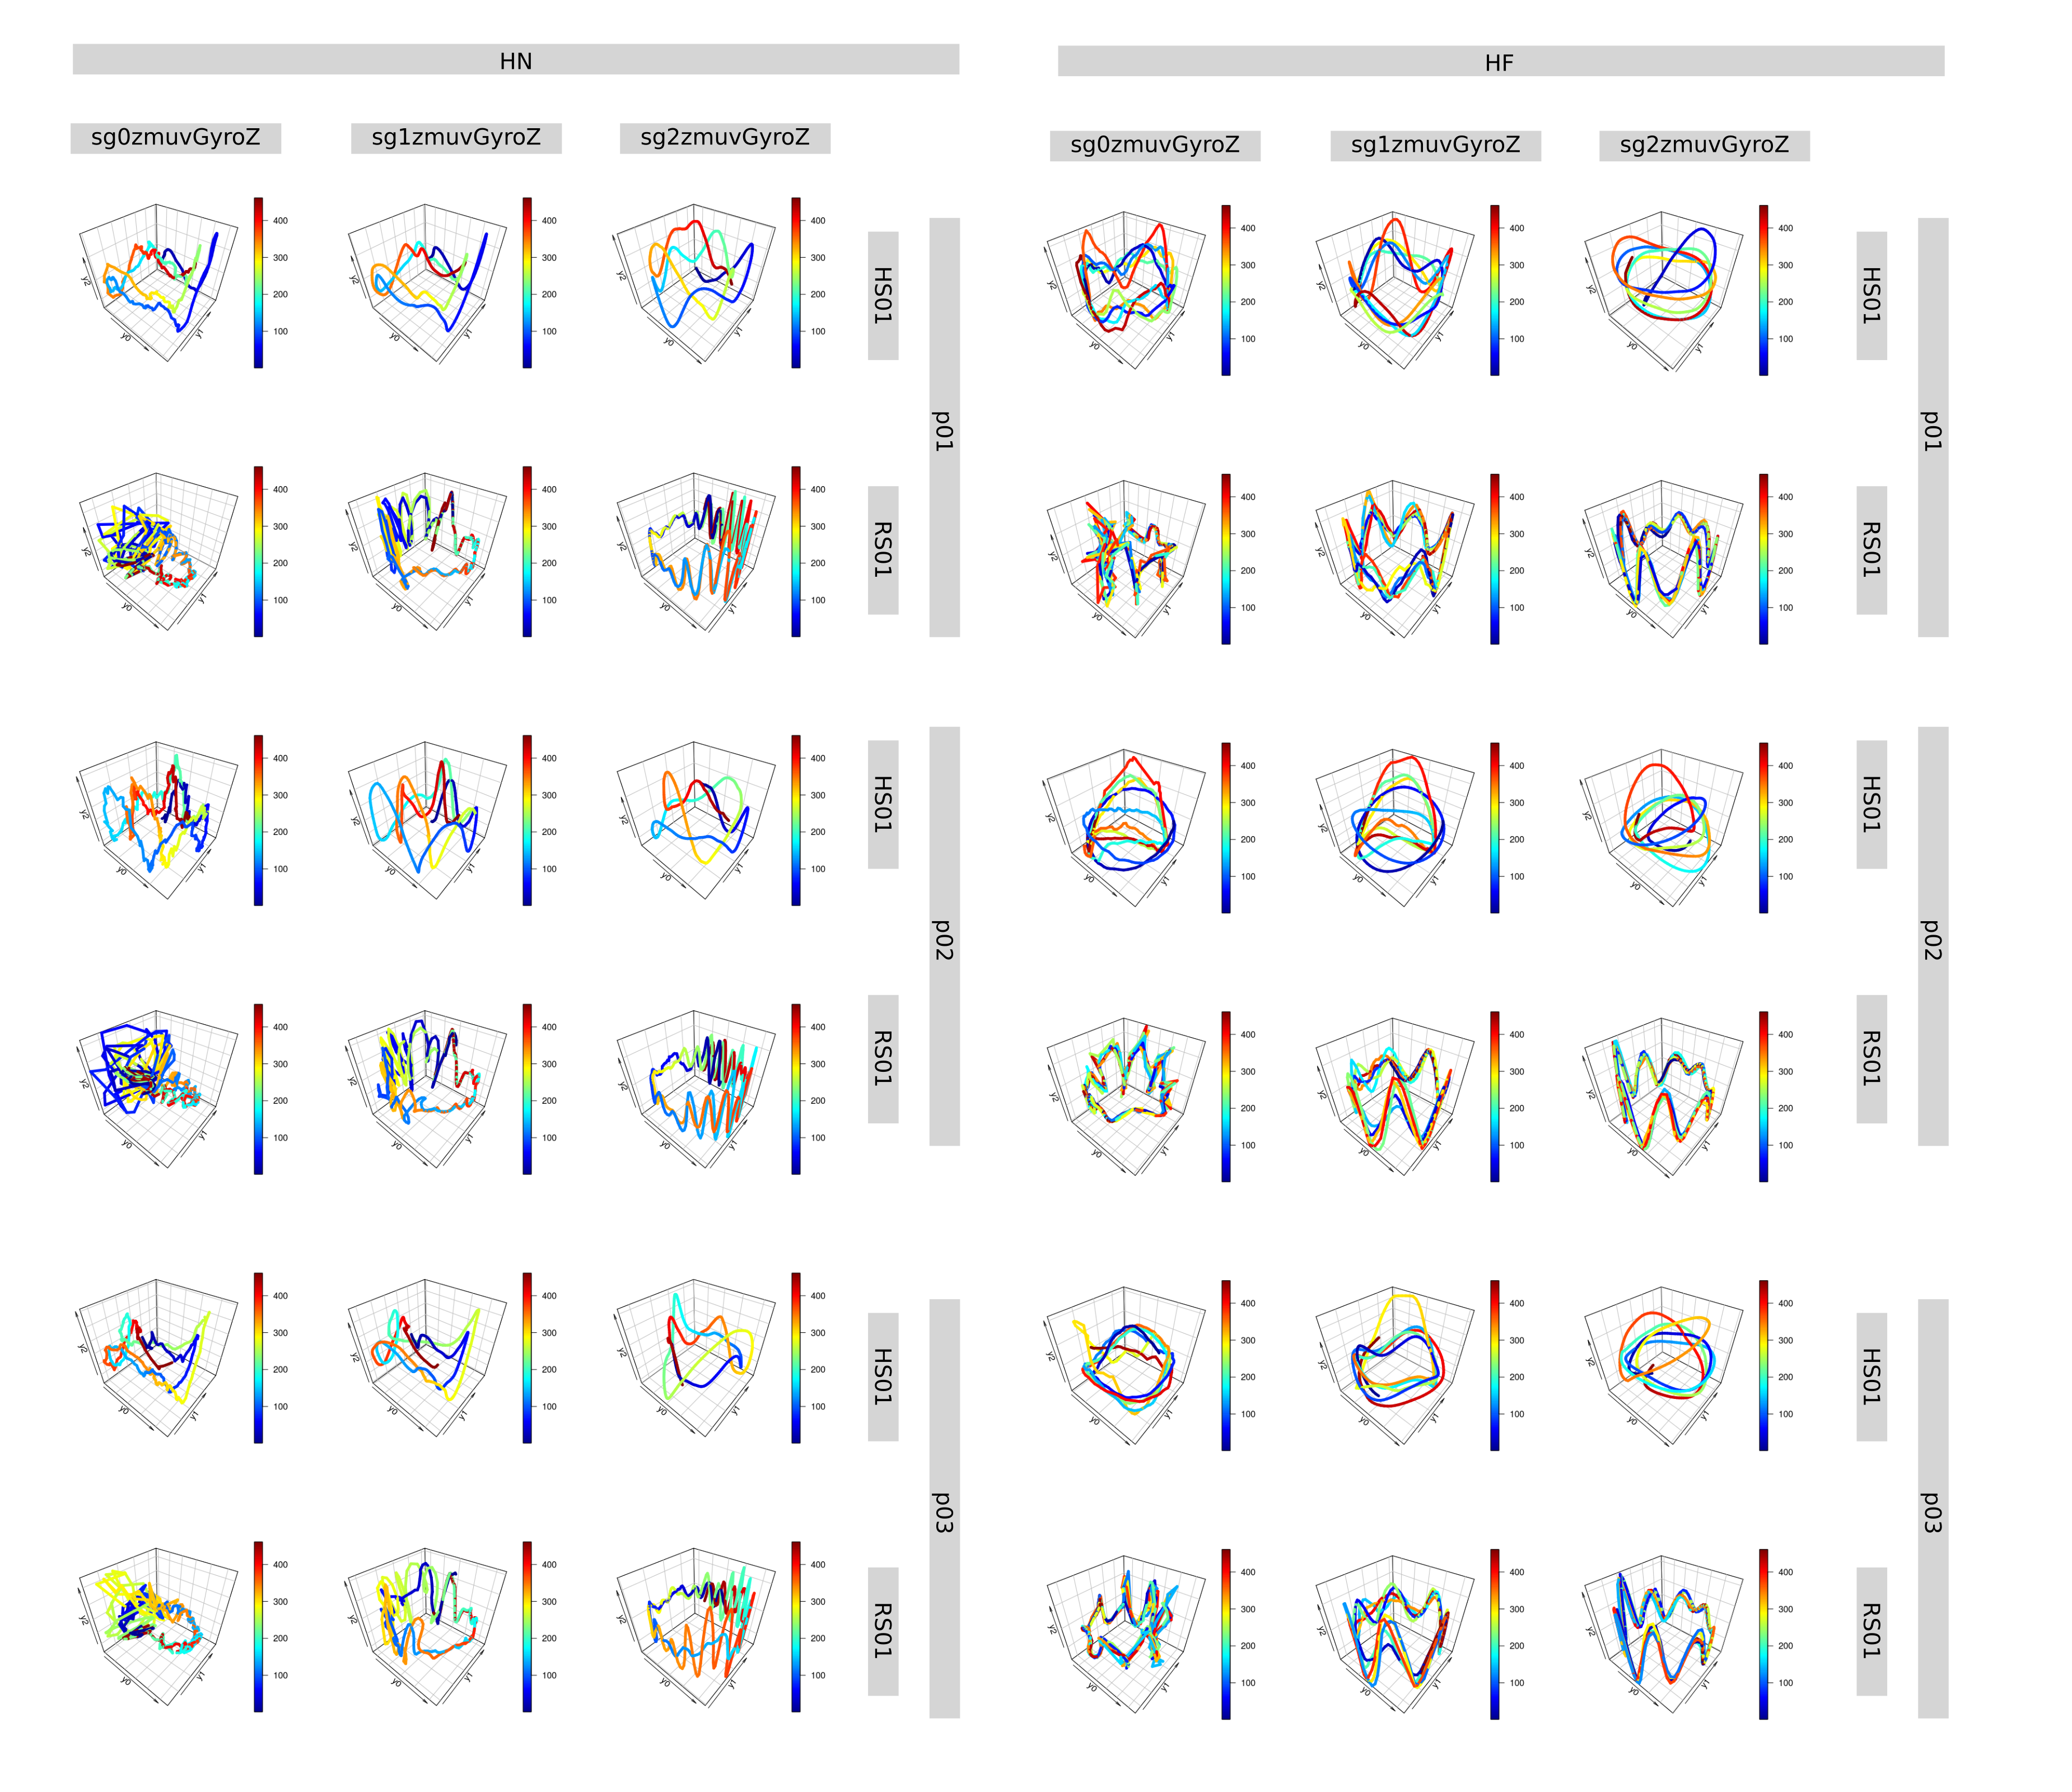
\includegraphics[width=1.0\textwidth]{rss_aH}
\caption{
	{\bf RSSs for horizontal arm movements.}
	Reconstructed state spaces for time series of Figure \ref{fig:tsH}.
	Reconstructed state spaces were computed with 
	embedding parameters $m=6$, $\tau=8$.
	R code to reproduce the figure is available from \cite{hwum2018}.
        }
    \label{fig:rss_aHw10}
\end{figure}
%%---------------------------------(FIGURE)------------------------------------
%%---------------------------------(FIGURE)-------------------------------------
\begin{figure}[!h]
\centering
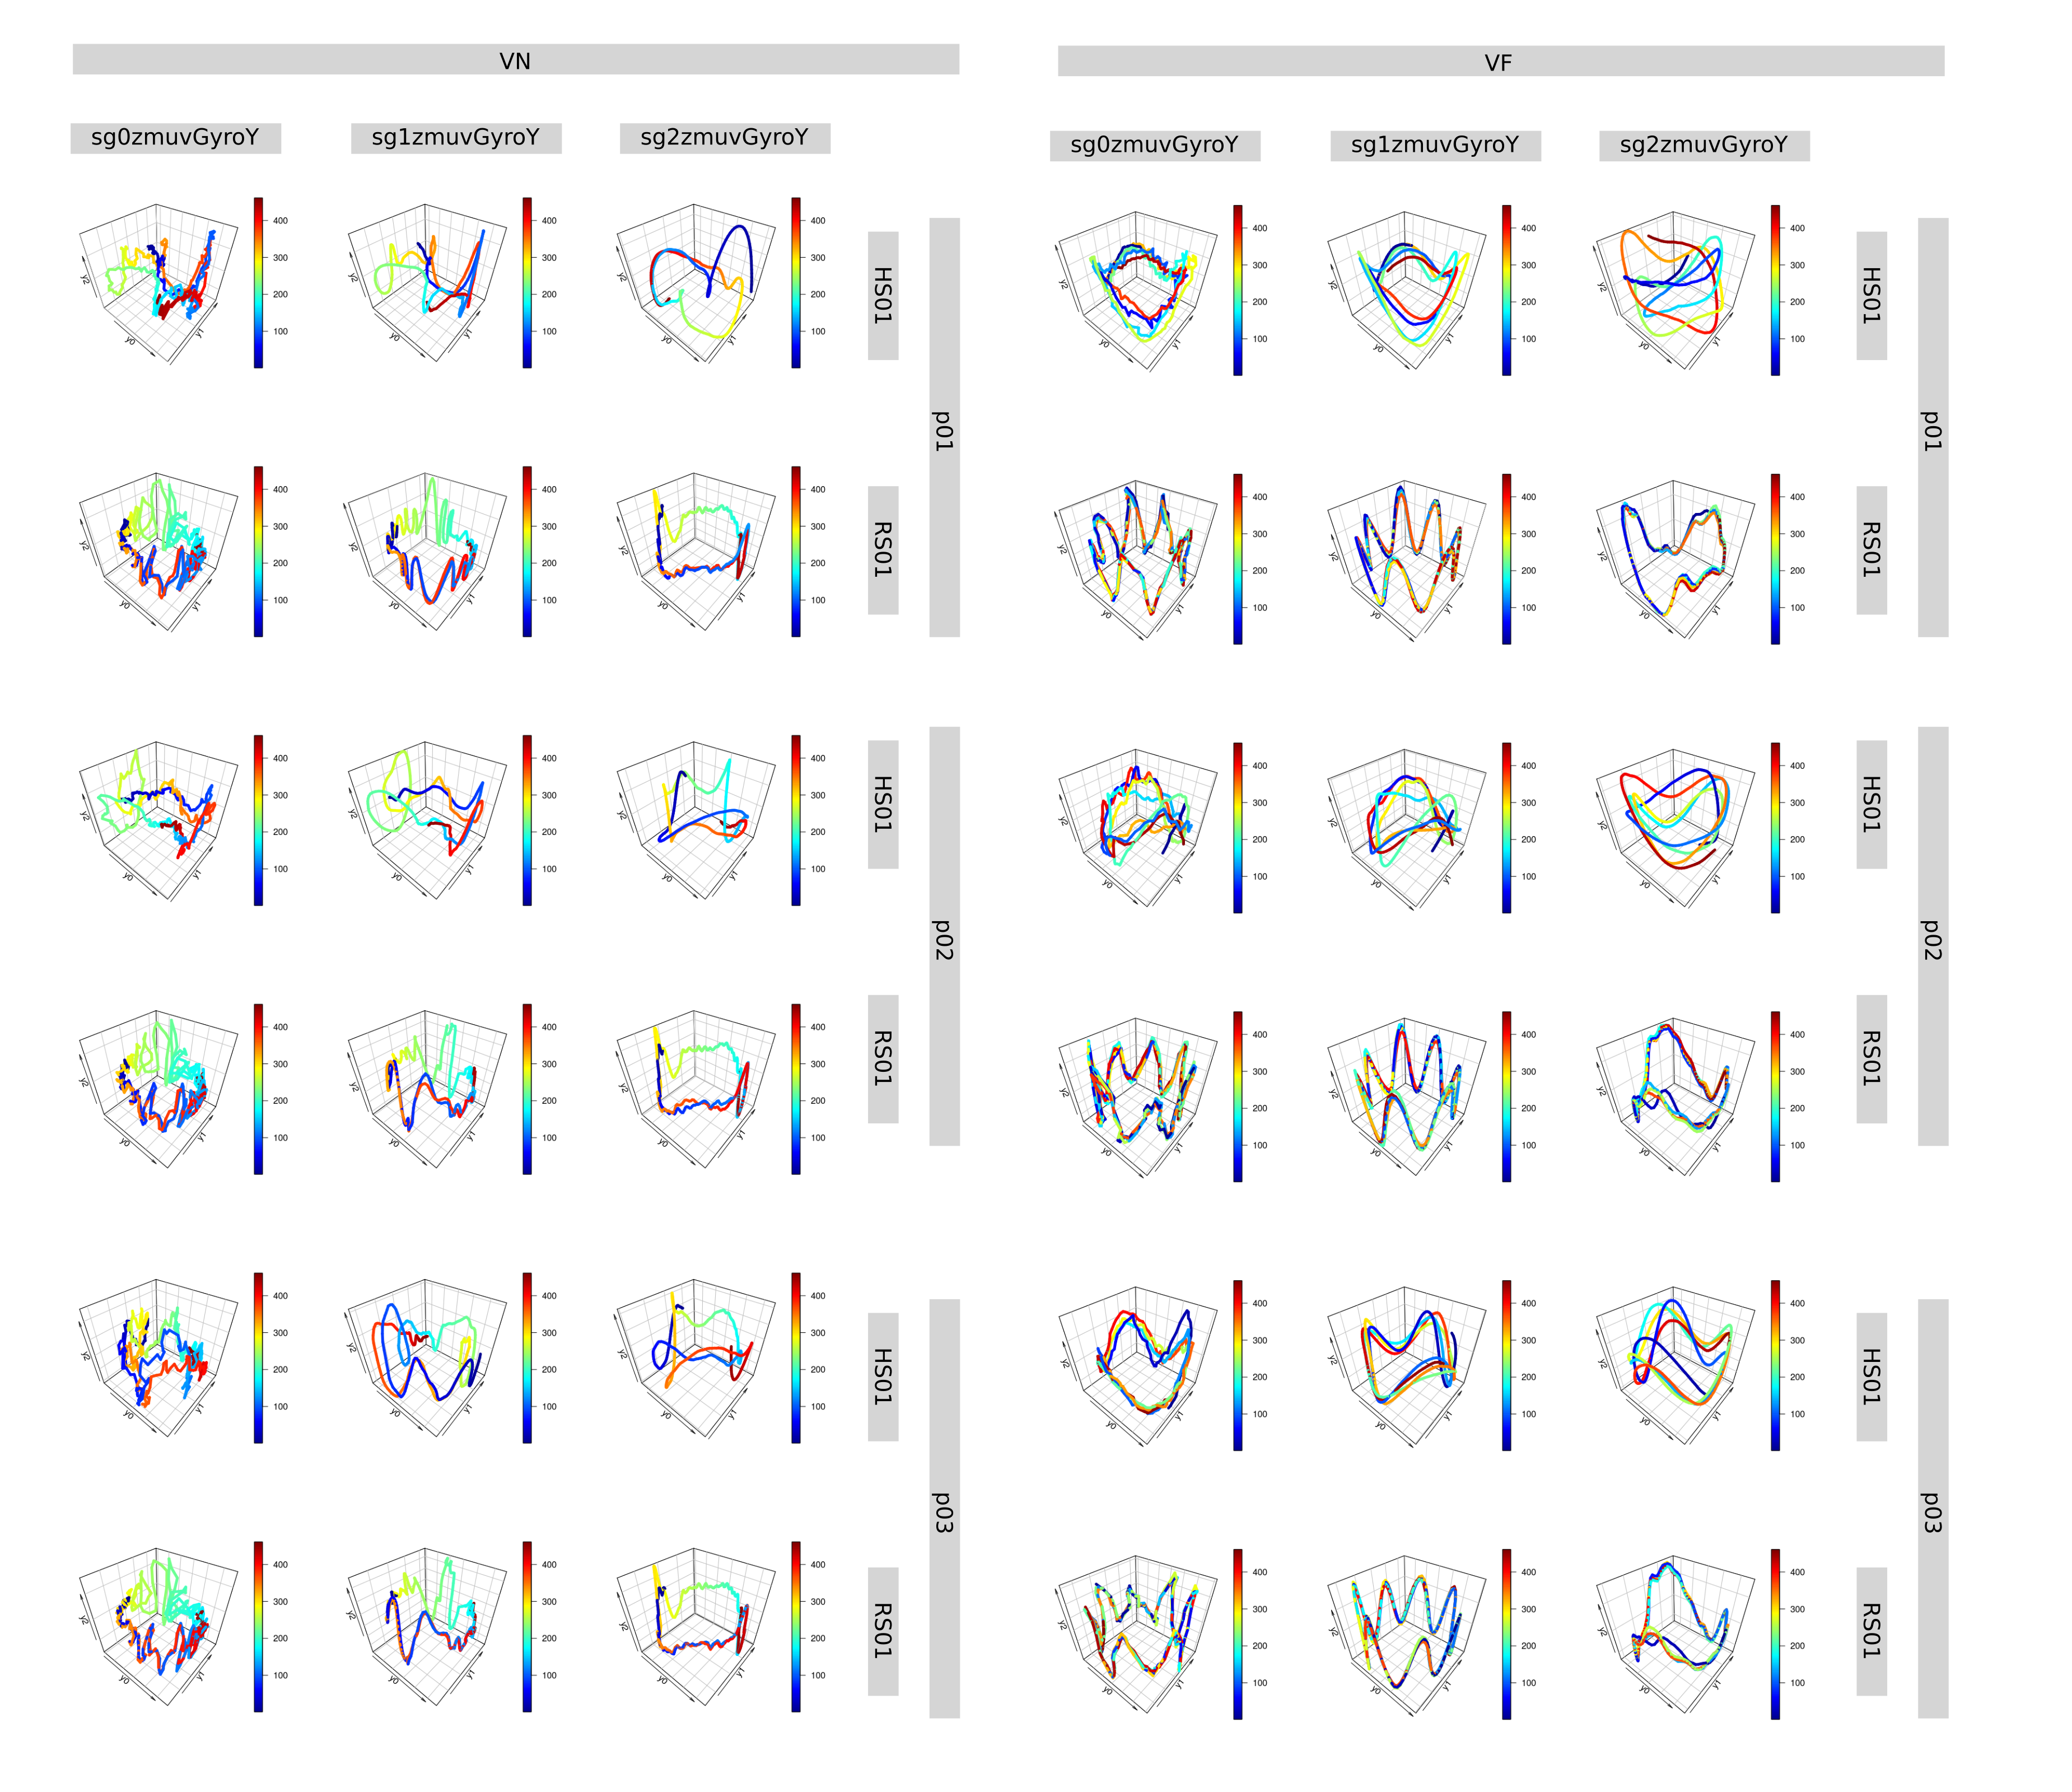
\includegraphics[width=1.0\textwidth]{rss_aV}
    \caption{
	{\bf RSSs for vertical arm movements.}
	Reconstructed state spaces for time series of Figure \ref{fig:tsV}.
	Reconstructed state spaces were computed with 
	embedding parameters $m=6$, $\tau=8$.
	R code to reproduce the figure is available from \cite{hwum2018}.
        }
    \label{fig:rss_aVw10}
\end{figure}
%%---------------------------------(FIGURE)------------------------------------

Evidently, it is easy to observe by eye the differences in each of the
trajectories in the reconstructed state spaces (Figs~\ref{fig:rss_aHw10}, \ref{fig:rss_aVw10}), 
however one might be not objective when quantifying those differences 
since those observation might vary from person to person.
With that in mind, we tried to objectively quantify those differences 
using euclidean distances between the origin to each of the points in the trajectories,
however these created suspicious metric, specially 
for trajectories which looked very messy.
With that in mind, we computed Recurrence Quantification Analysis
to objectively quantify the differences in each of the cases of
the time series.







%%%%%%%%%%%%%%%%%%%%%%%%%%%%%%%%%%%%%%%%%%%%%%%%%%%%%%%%%%%%%%%%%%%%%%%%%%%%%%%
%%%%%%%%%%%%%%%%%%%%%%%%%%%%%%%%%%%%%%%%%%%%%%%%%%%%%%%%%%%%%%%%%%%%%%%%%%%%%%%
\subsection{RPs and RQA for time series in the context of human-robot interaction}

\subsubsection{Recurrences Plots}
Considering the time series of Figs~\ref{fig:tsH} and \ref{fig:tsV}, 
we computed its Recurrence Plots
for horizontal arm movements (Fig~\ref{fig:rp_aH}) and
for vertical arm movements (Fig~\ref{fig:rp_aV}) 
using the average embedding parameters ($m=6$, $\tau=8$) 
and an recurrence threshold of $\epsilon=1$.
With regard to the selection of recurrence threshold,
Marwan et al. \cite{marwan2011} pointed out that choosing an appropriate recurrence threshold 
is crucial to get meaningful representations in RPs, however, 
for our work where quantifying movement variability is our aim,
we give little importance to the selection of the recurrence threshold as
as long as it is able to represent the dynamical transitions 
in each of the time series.

As similar as with the Reconstructed State Spaces, 
the differences in the RPs can be easily noticed by eye 
for different conditions of the time series (Figs~\ref{fig:rp_aV}, Fig~\ref{fig:rp_aH}),
which lead us to apply Recurrence Quantification Analysis 
to have an objective quantification of each of the time series.
%%---------------------------------(FIGURE)-------------------------------------
\begin{figure}[!h]
\centering
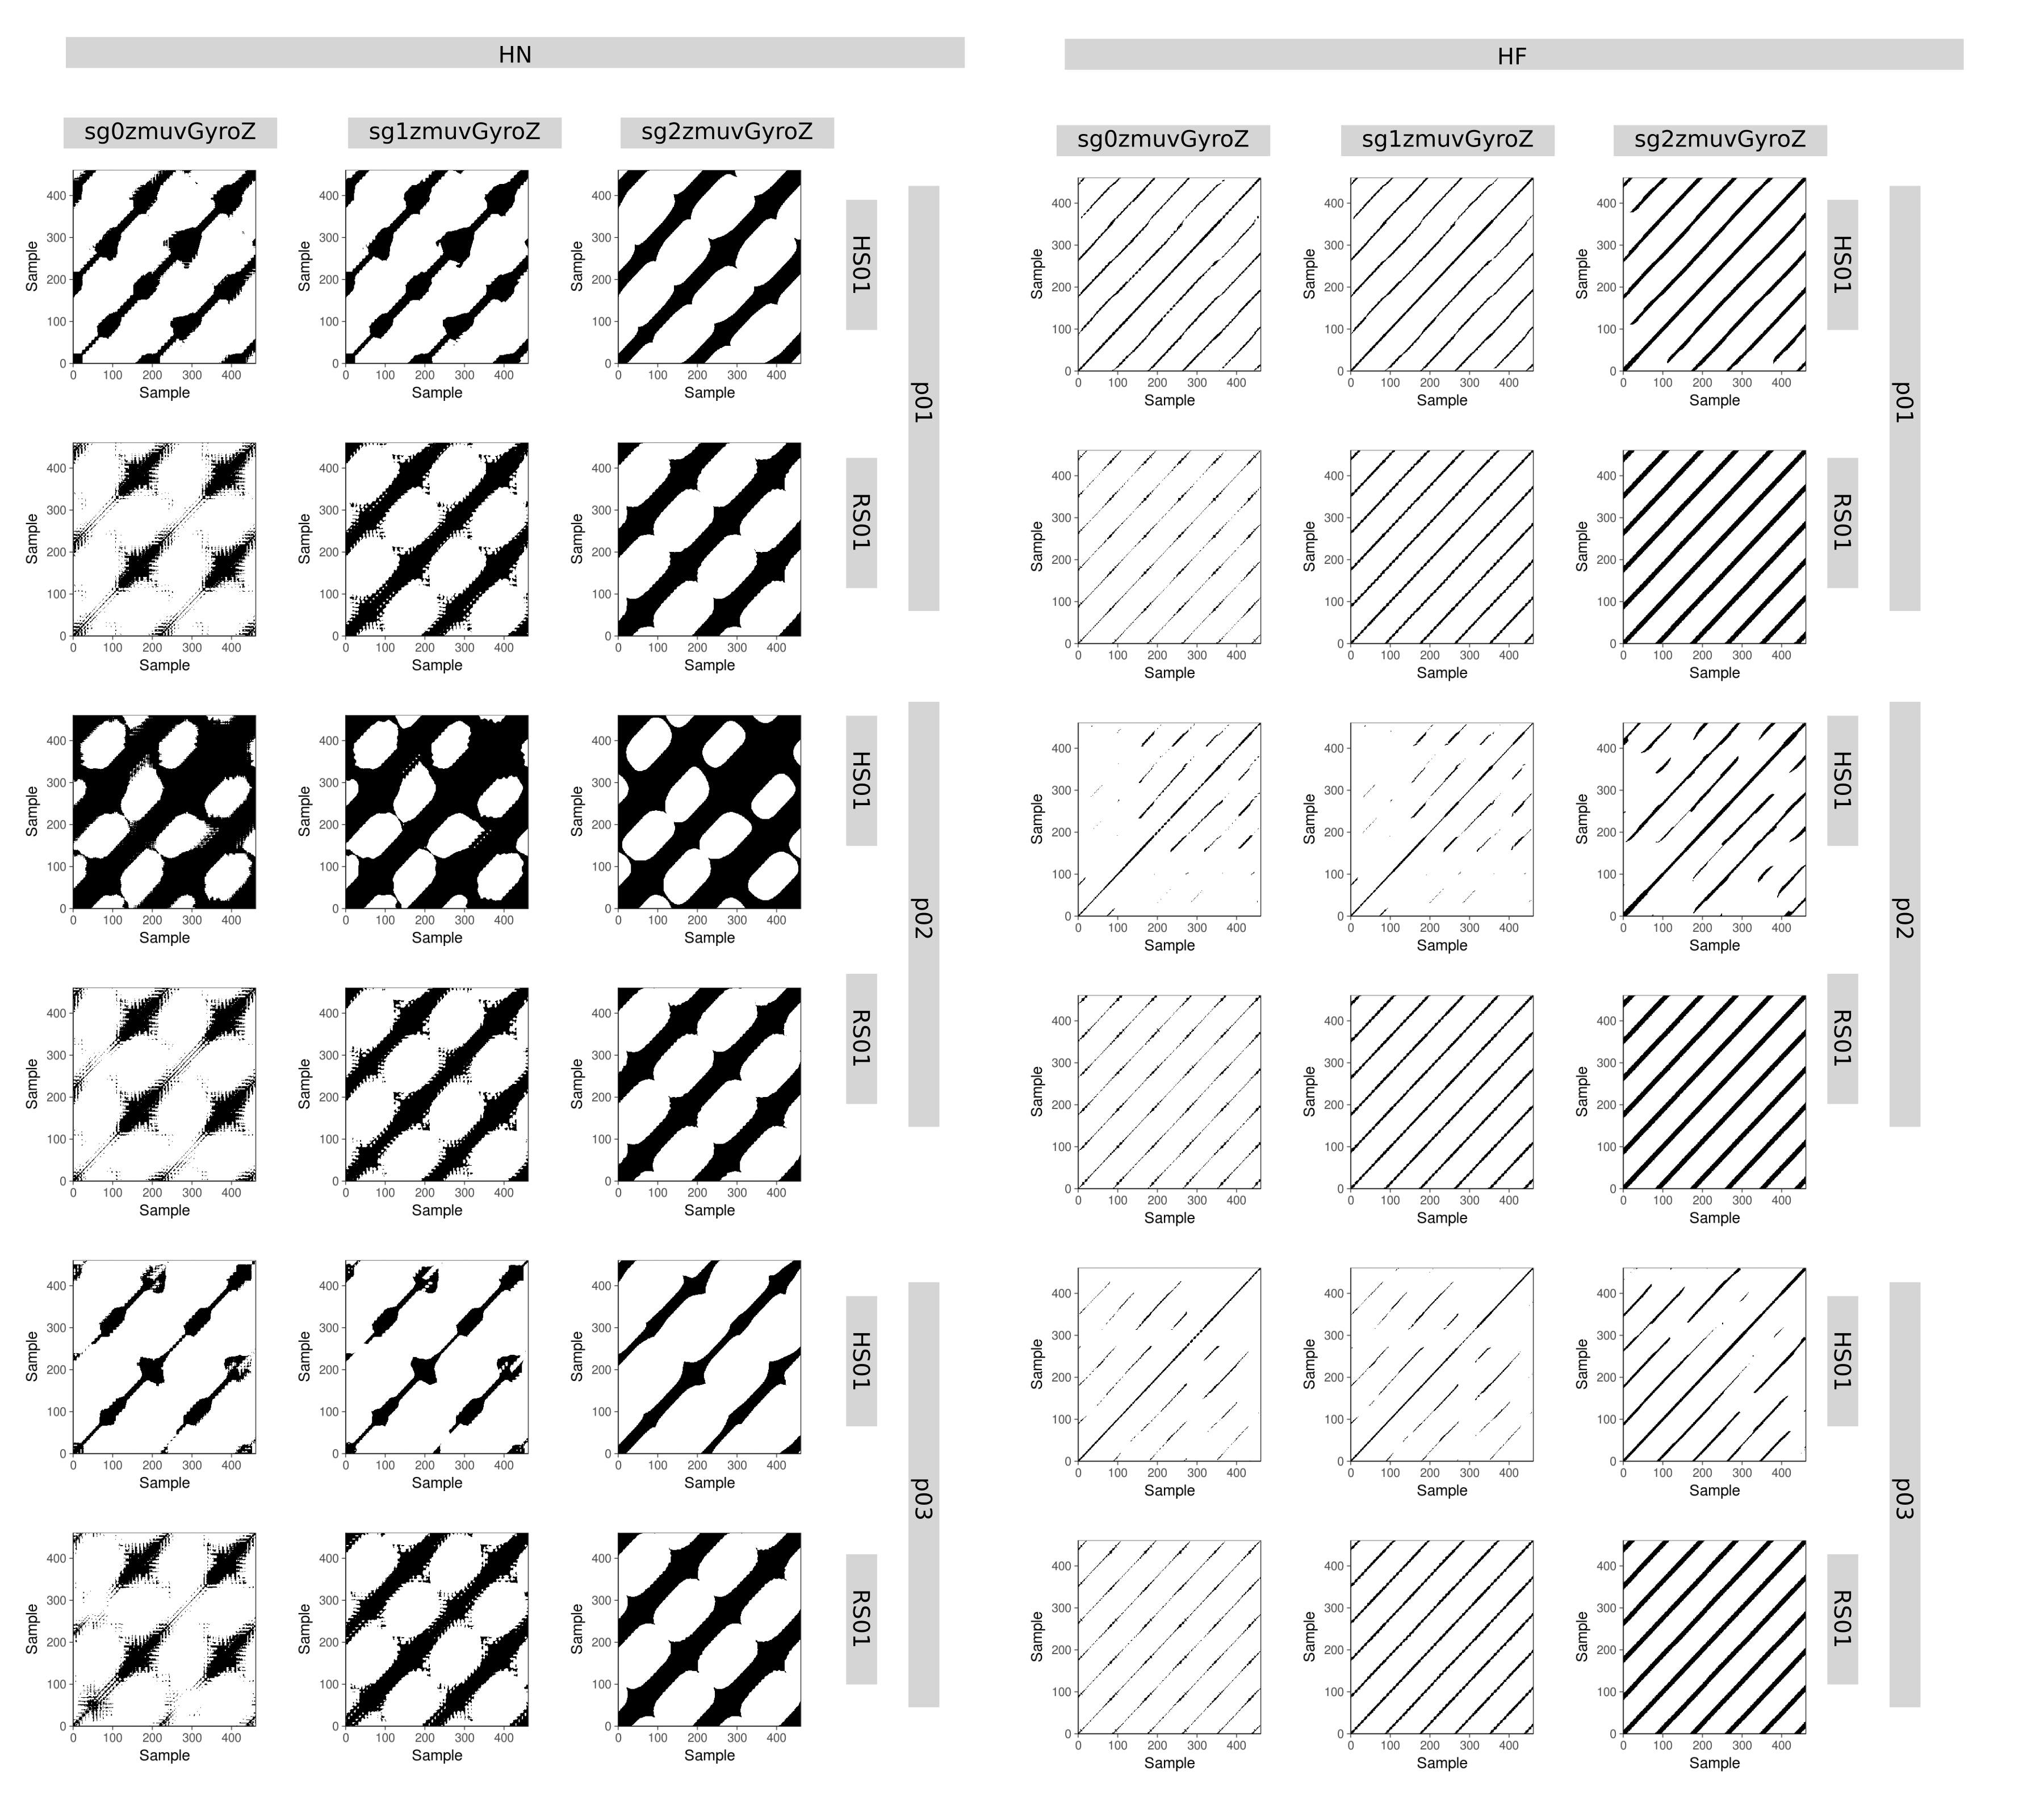
\includegraphics[width=1.0\textwidth]{rp_aH}
\caption{
	{\bf RPs for horizontal arm movements.}	
	Recurrence plots were computed with 
	embedding parameters $m=6$, $\tau=8$ and $\epsilon=1$.
	R code to reproduce the figure is available from \cite{hwum2018}.
        }
    \label{fig:rp_aH}
\end{figure}
%%---------------------------------(FIGURE)------------------------------------
%%---------------------------------(FIGURE)-------------------------------------
\begin{figure}[!h]
\centering
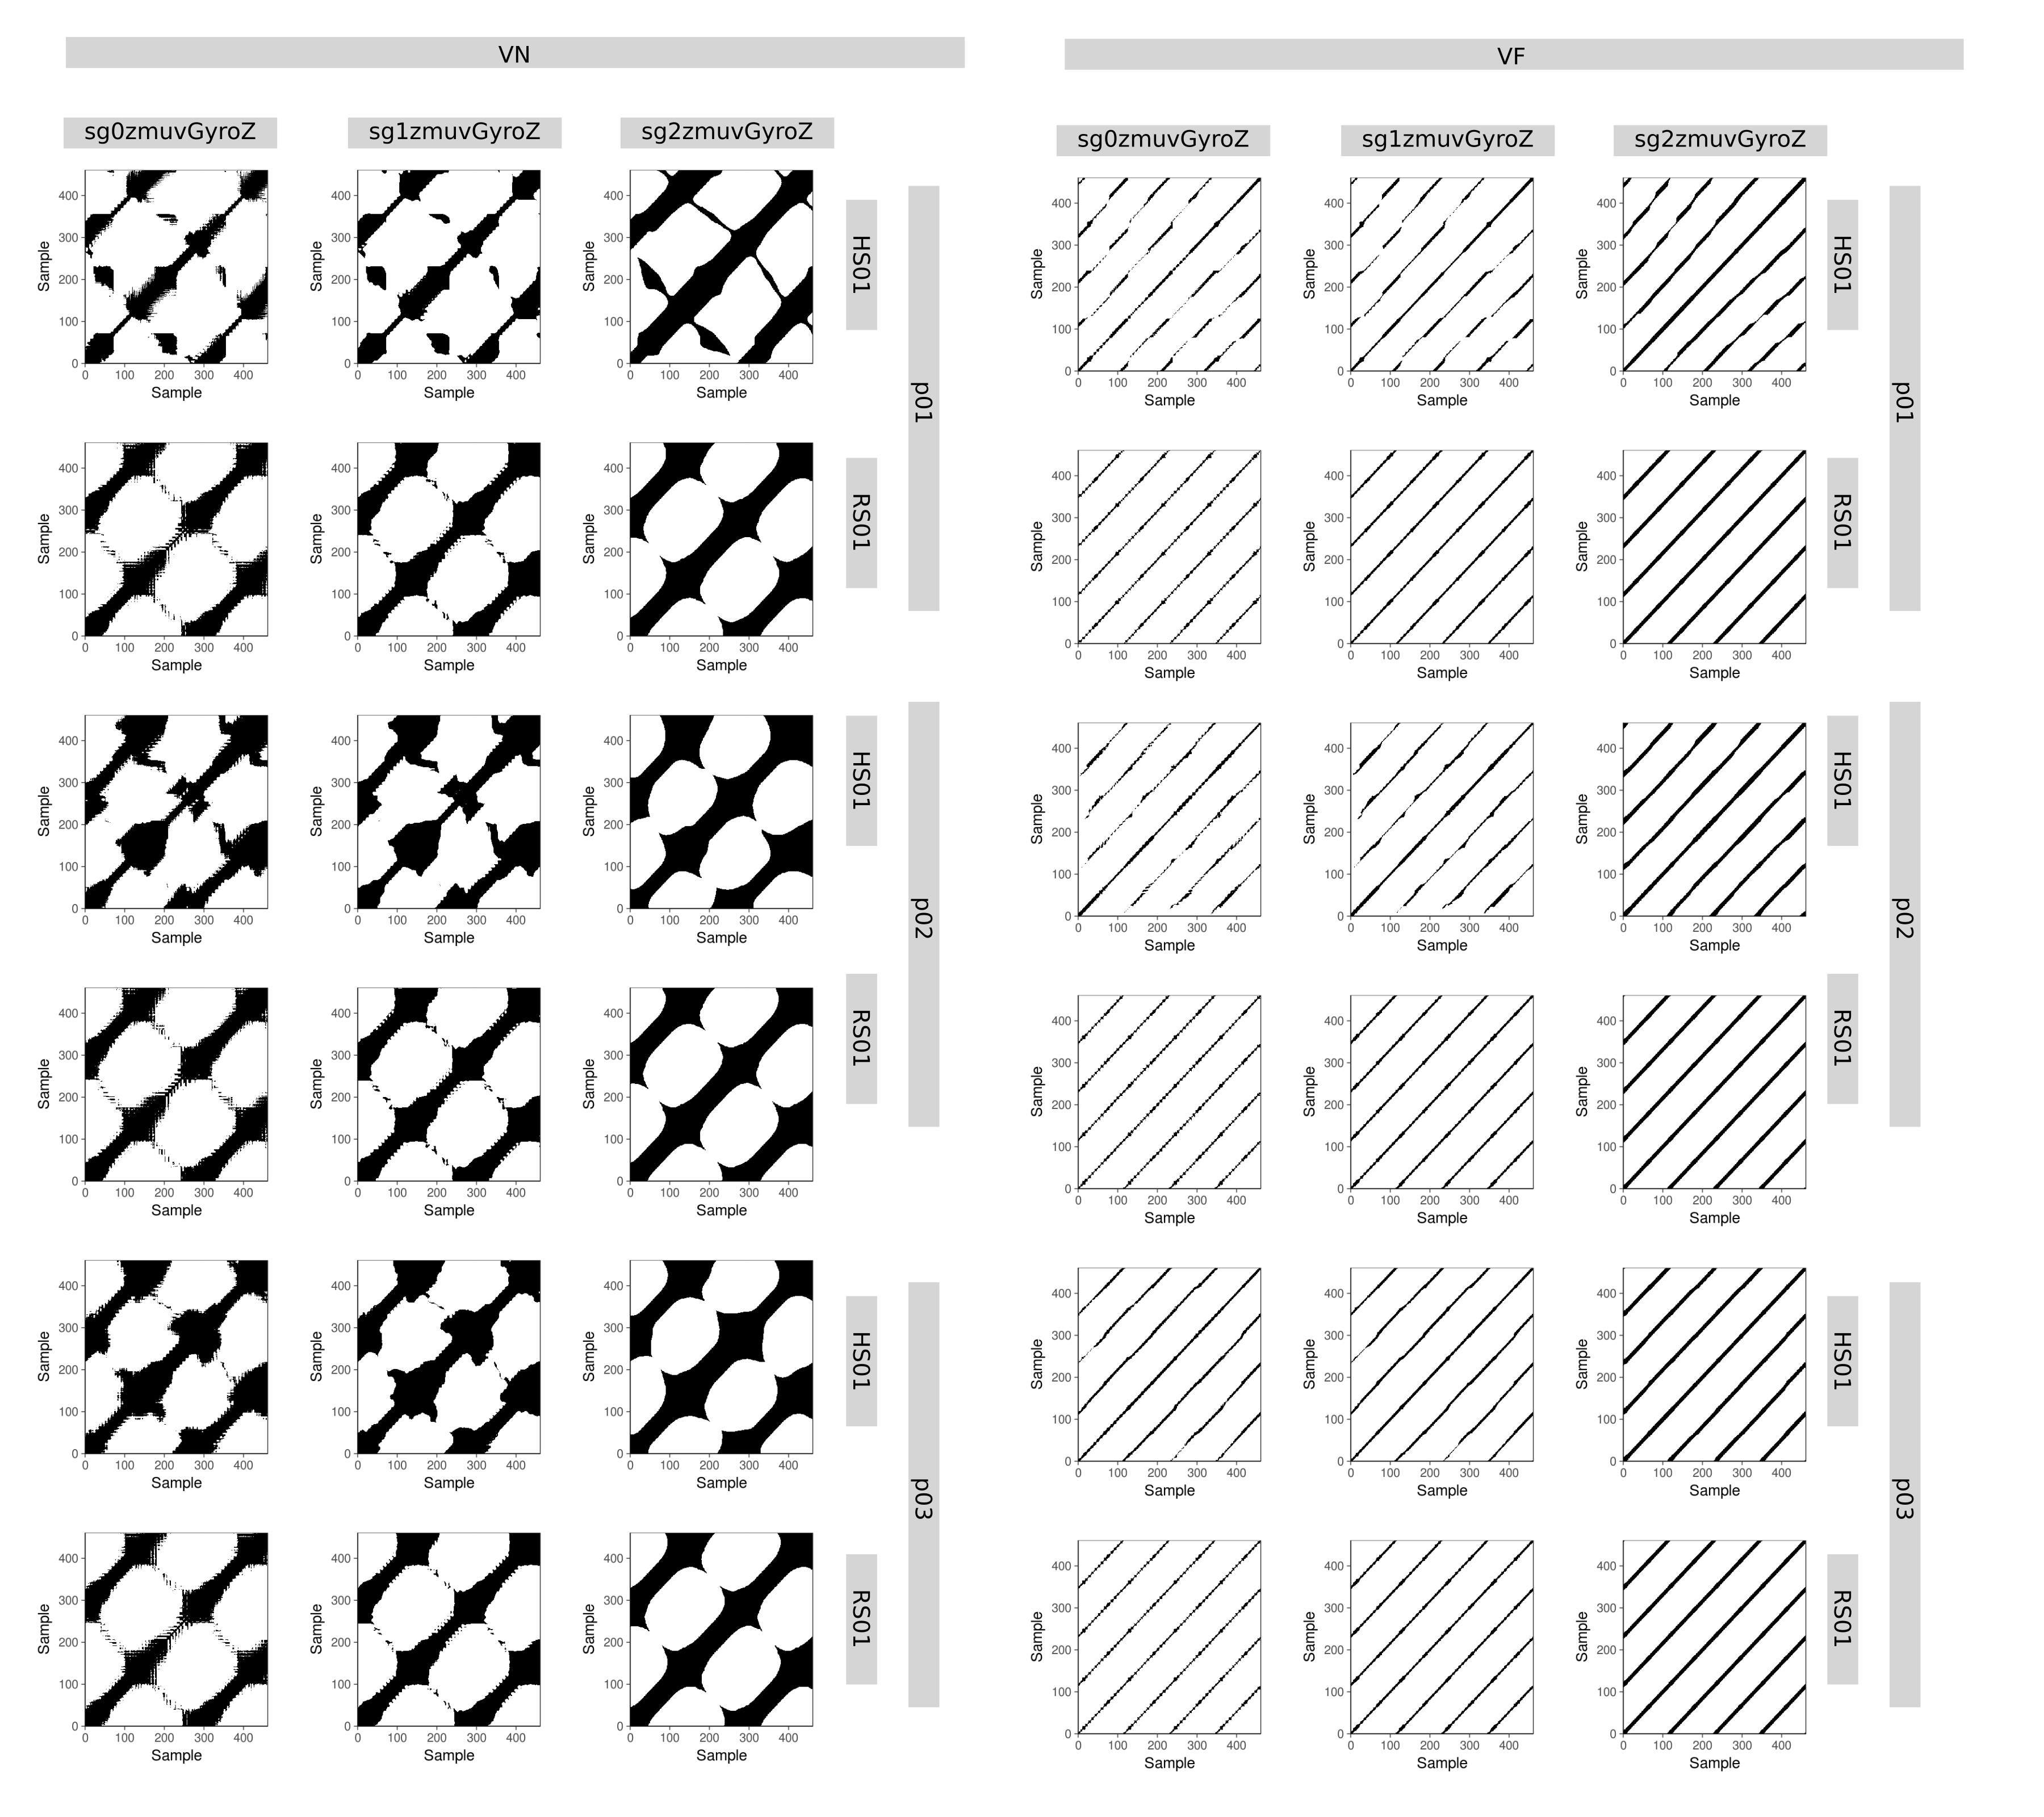
\includegraphics[width=1.0\textwidth]{rp_aV}
\caption{
	{\bf RPs for vertical arm movements.}	
	Recurrence plots were computed with 
	embedding parameters $m=6$, $\tau=8$ and $\epsilon=1$.
	R code to reproduce the figure is available from \cite{hwum2018}.
        }
    \label{fig:rp_aV}
\end{figure}
%%---------------------------------(FIGURE)------------------------------------








\subsubsection{Recurrence Quantification Analysis}
RPs provided pattern formations for each of the time series 
conditions (Figs~\ref{fig:rp_aH} and \ref{fig:rp_aV}).
Hence, the following four metrics of RQA metrics 
(REC, DET, RATIO and ENTR) are computed:

\subsubsection*{REC values}
In Figs~\ref{fig:rec_aH} and \ref{fig:rec_aV} can be seen that REC values 
are more spread for HN than HF movements with data coming from HS01 sensor. 
In contrast, REC values appear to be constant and present 
little variation for both HN and HF movements 
with data from the sensor attached to the humanoid robot RS01.
With regard to the increase of smoothness of data (sg0zmuvGyroZ, sg1zmuvGyroZ and sg2zmuvGyroZ), 
REC values present little variation as the smoothness is increasing for data 
from HS01 and REC values more similar as the smoothness is increasing for data from RS01.
%%---------------------------------(FIGURE)-------------------------------------
\begin{figure}[!h]
\centering
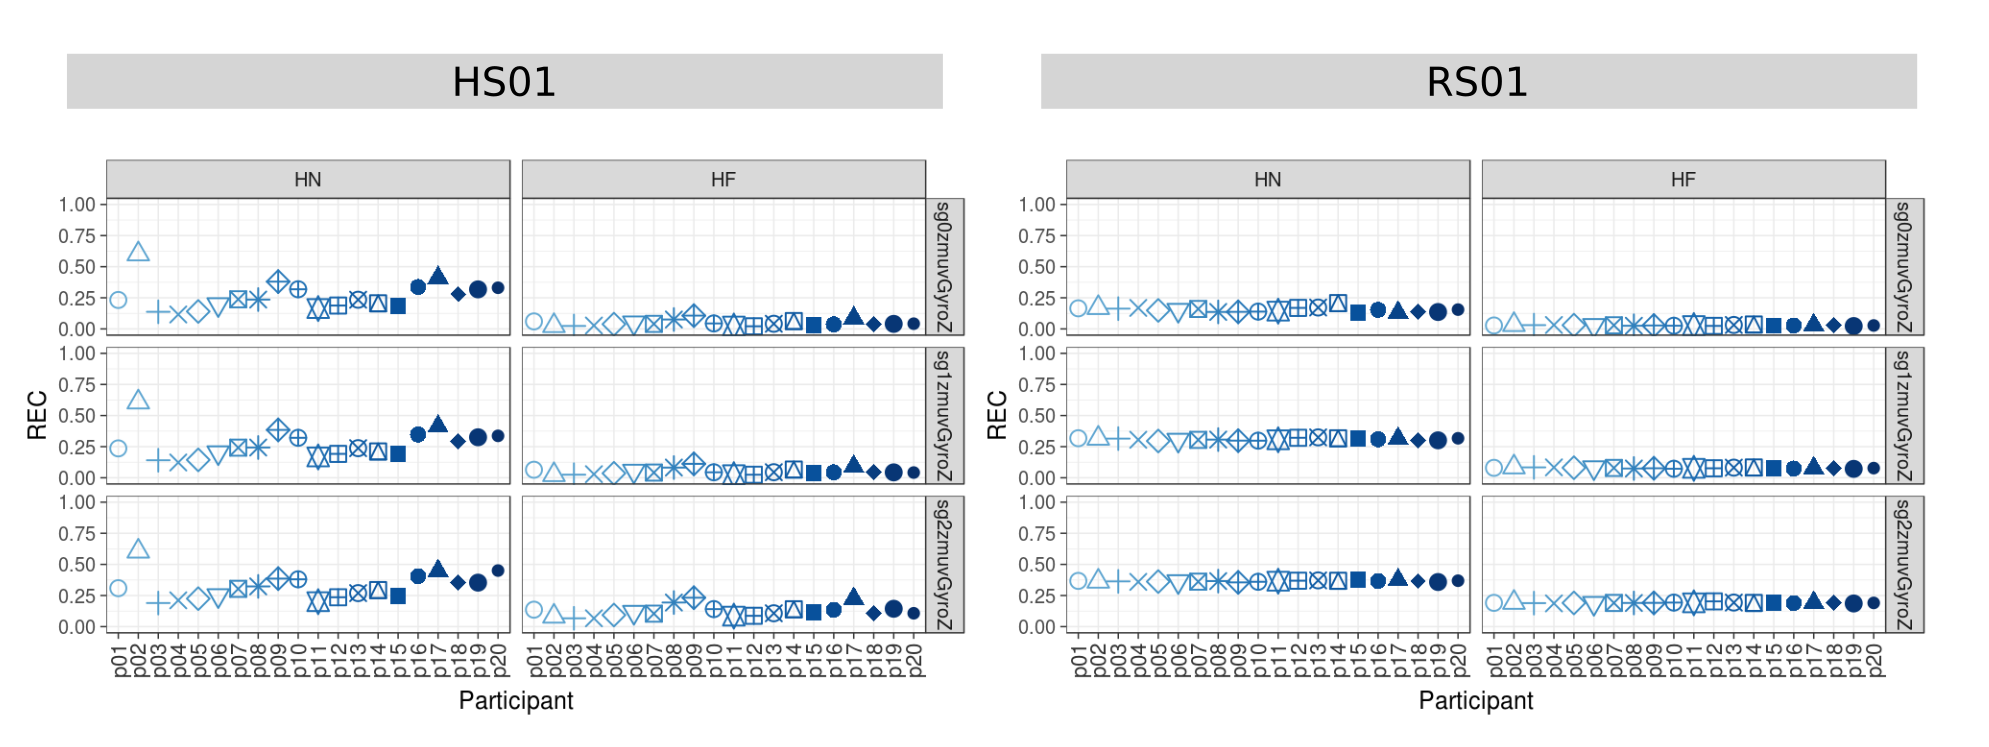
\includegraphics[width=1.0\textwidth]{rec_aH}
    \caption{
	{\bf REC values for horizontal arm movements.}	
	REC values (representing \% of black dots in the RPs) for 
	20 participants performing HN and HF movements
	with sensors HS01, RS01 and three smoothed-normalised axis 
	of GyroZ (sg0zmuvGyroZ, sg1zmuvGyroZ and sg2zmuvGyroZ).
	REC values were computed with 
	embedding parameters $m=6$, $\tau=8$ and $\epsilon=1$
	R code to reproduce the figure is available from \cite{hwum2018}.
        }
    \label{fig:rec_aH}
\end{figure}
%%---------------------------------(FIGURE)------------------------------------
%%---------------------------------(FIGURE)-------------------------------------
\begin{figure}[!h]
\centering
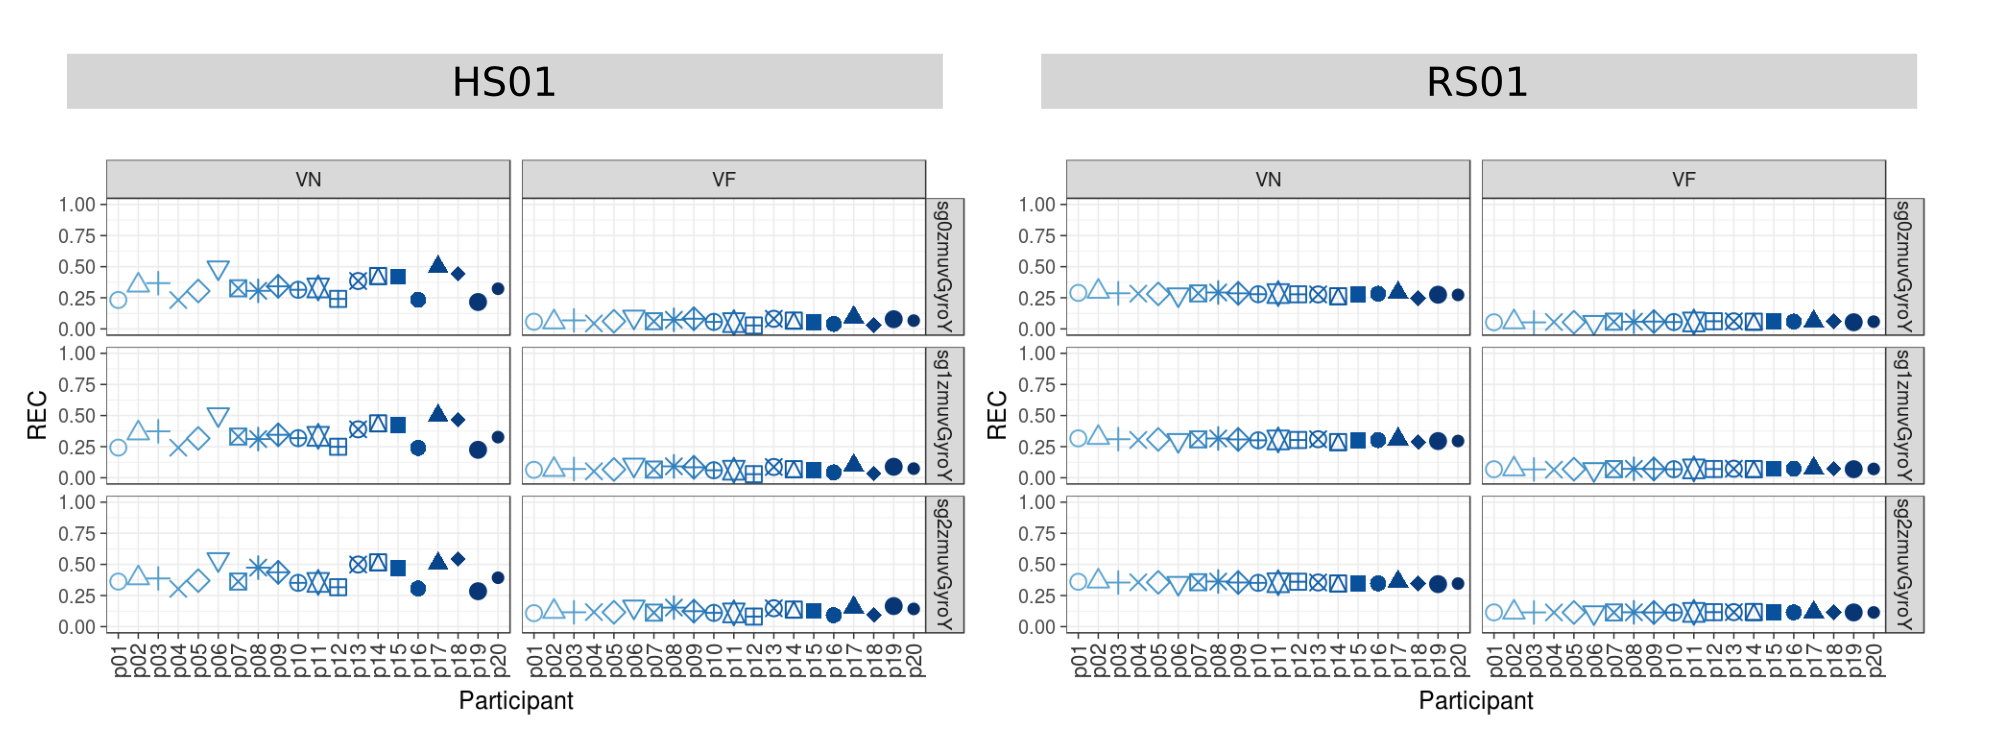
\includegraphics[width=1.0\textwidth]{rec_aV}
    \caption{
	{\bf REC values for vertical arm movements.}	
	REC values (representing \% of black dots in the RPs) for 
	20 participants performing VN and VF movements
	with sensors HS01, RS01 and three smoothed-normalised axis 
	of GyroY (sg0zmuvGyroY, sg1zmuvGyroY and sg2zmuvGyroY).
	REC values were computed with 
	embedding parameters $m=6$, $\tau=8$ and $\epsilon=1$.
	R code to reproduce the figure is available from \cite{hwum2018}.
        }
    \label{fig:rec_aV}
\end{figure}
%%---------------------------------(FIGURE)------------------------------------







\subsubsection*{DET values}
Little can be said with regard to the variation of DET values
as these change very little even for type of movement or type of sensor
(Figs~\ref{fig:det_aH} and \ref{fig:det_aV}).
With regard to the smoothness of time series, DET values appear to be more similar 
as the smoothness of the data is increasing.
%%---------------------------------(FIGURE)-------------------------------------
\begin{figure}[!h]
\centering
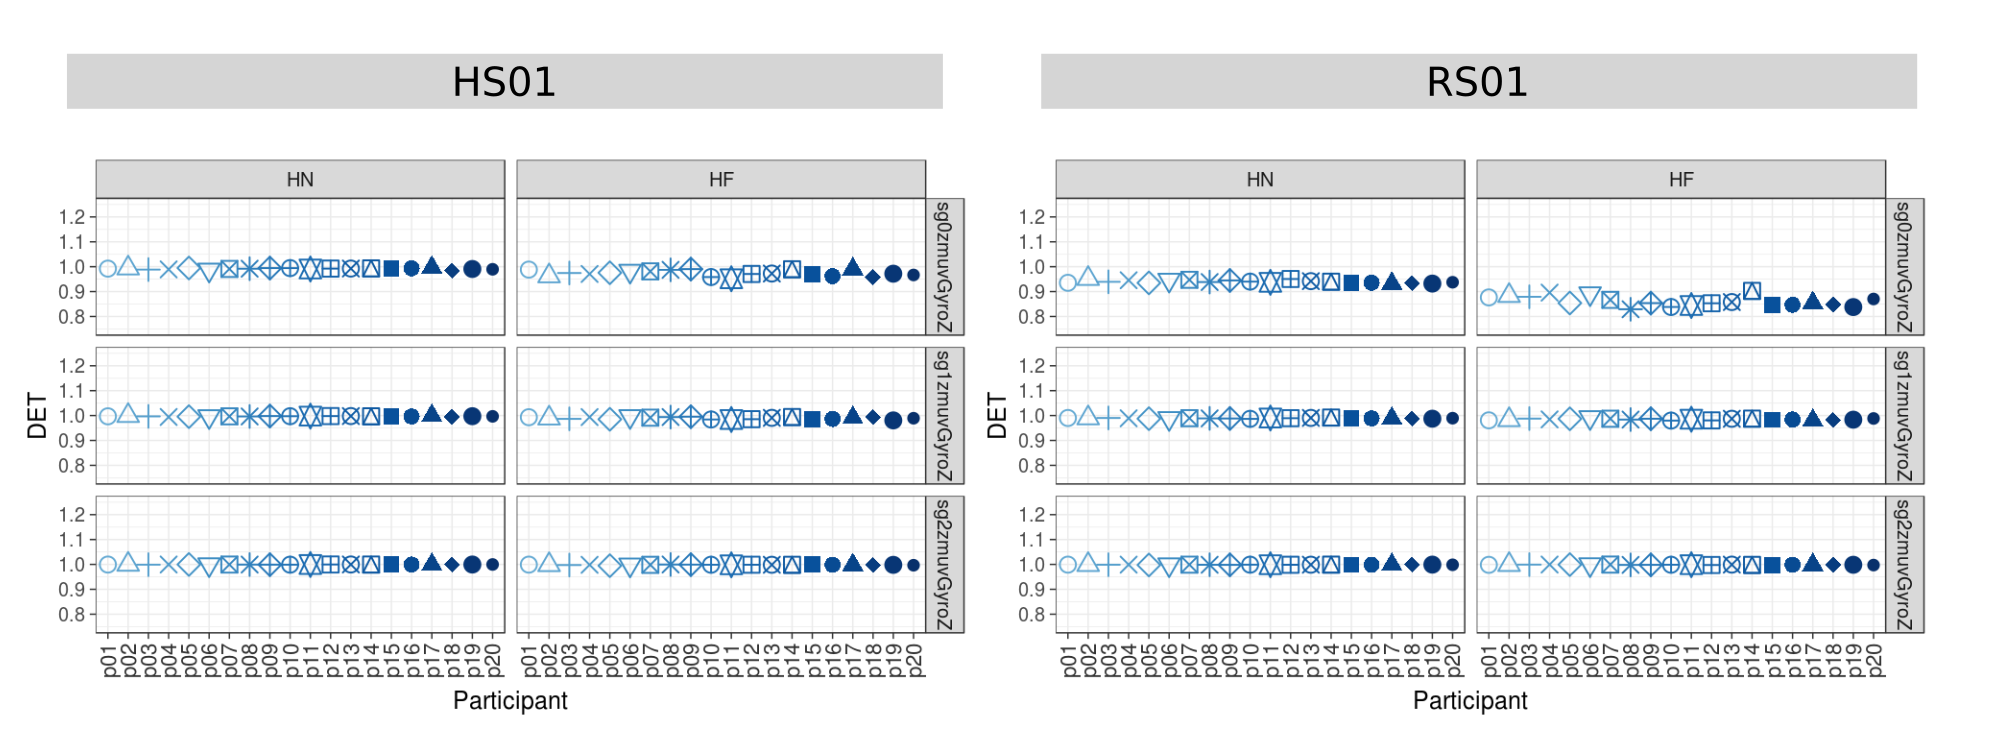
\includegraphics[width=1.0\textwidth]{det_aH}
    \caption{
	{\bf DET values for horizontal arm movements.}	
    	DET values (representing predictability and organisation of the RPs) for 
	20 participants performing HN and HF movements
	with sensors HS01, RS01 and three smoothed-normalised axis 
	of GyroZ (sg0zmuvGyroZ, sg1zmuvGyroZ and sg2zmuvGyroZ).
	DET values were computed with 
	embedding parameters $m=6$, $\tau=8$ and $\epsilon=1$.
	R code to reproduce the figure is available from \cite{hwum2018}.
        }
    \label{fig:det_aH}
\end{figure}
%%---------------------------------(FIGURE)------------------------------------
%%---------------------------------(FIGURE)-------------------------------------
\begin{figure}[!h]
\centering
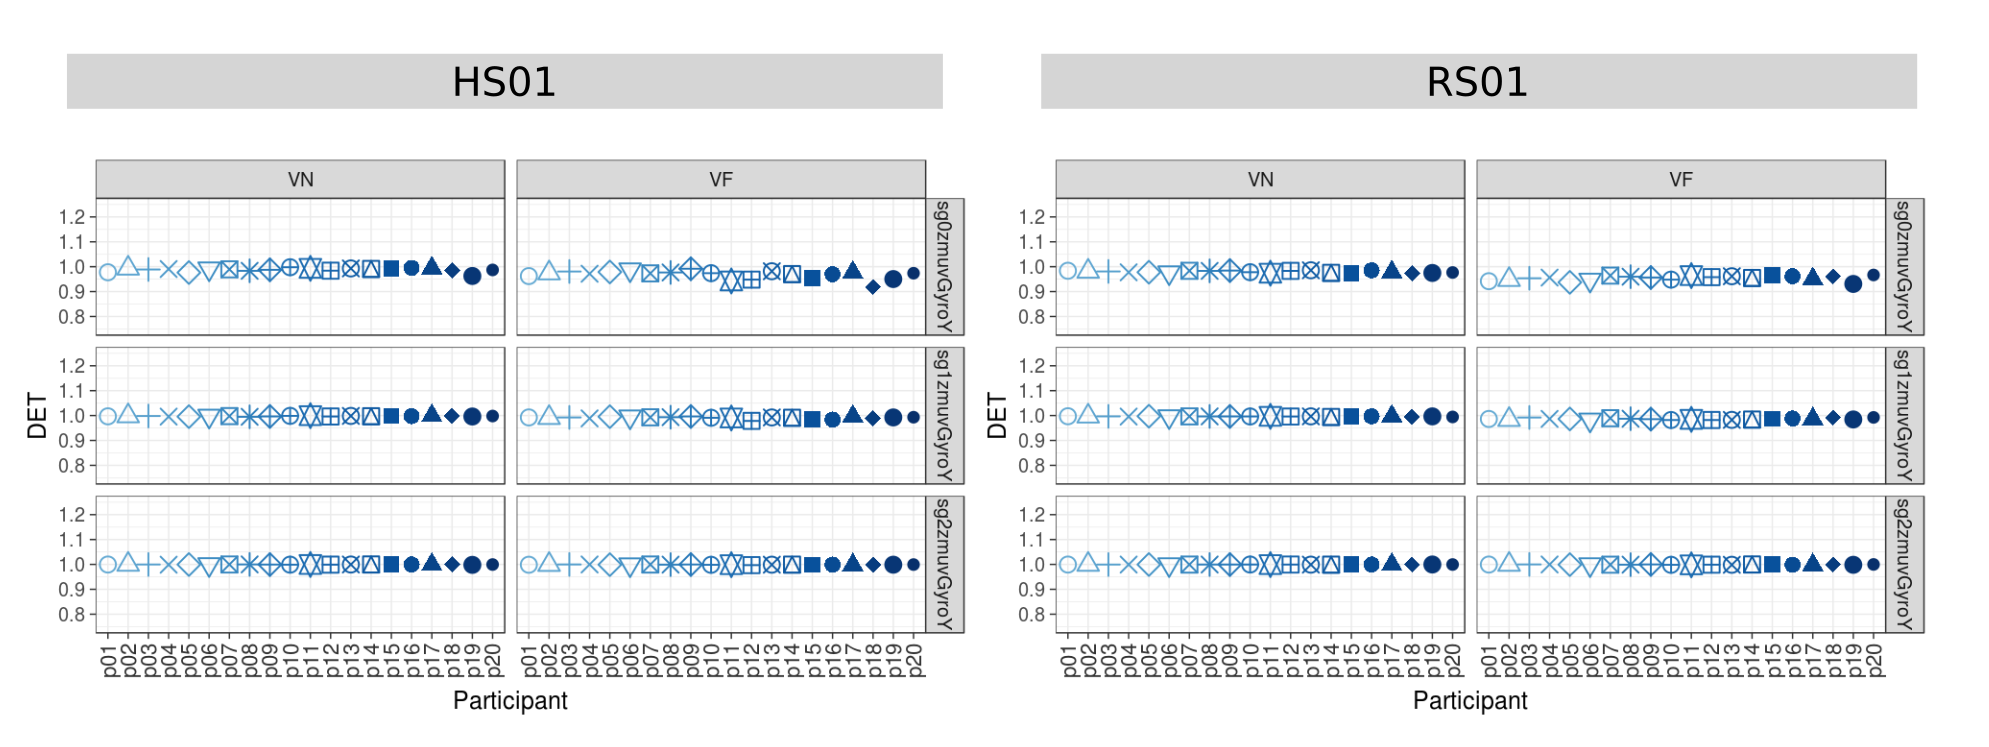
\includegraphics[width=1.0\textwidth]{det_aV}
    \caption{
	{\bf DET values for vertical arm movements.}	
    	DET values (representing predictability and organisation of the RPs) for 
	20 participants performing VN and VF movements
	with sensors HS01, RS01 and three smoothed-normalised axis 
	of GyroY (sg0zmuvGyroY, sg1zmuvGyroY and sg2zmuvGyroY).
	DET values were computed with 
	embedding parameters $m=6$, $\tau=8$ and $\epsilon=1$.
	R code to reproduce the figure is available from \cite{hwum2018}.
        }
    \label{fig:det_aV}
\end{figure}
%%---------------------------------(FIGURE)------------------------------------







\subsubsection*{RATIO values}
RATIO values for HN movements vary less than HF movements for HS01 sensor 
which is similar behaviour of RATIO values for RS01 sensors 
in both vertical and horizontal movements (Figs~\ref{fig:ratio_aH} and \ref{fig:ratio_aV}).
It can also noticed a decrease of variation in RATIO values as the smoothness of the signal is increasing.
%%---------------------------------(FIGURE)-------------------------------------
\begin{figure}[!h]
\centering
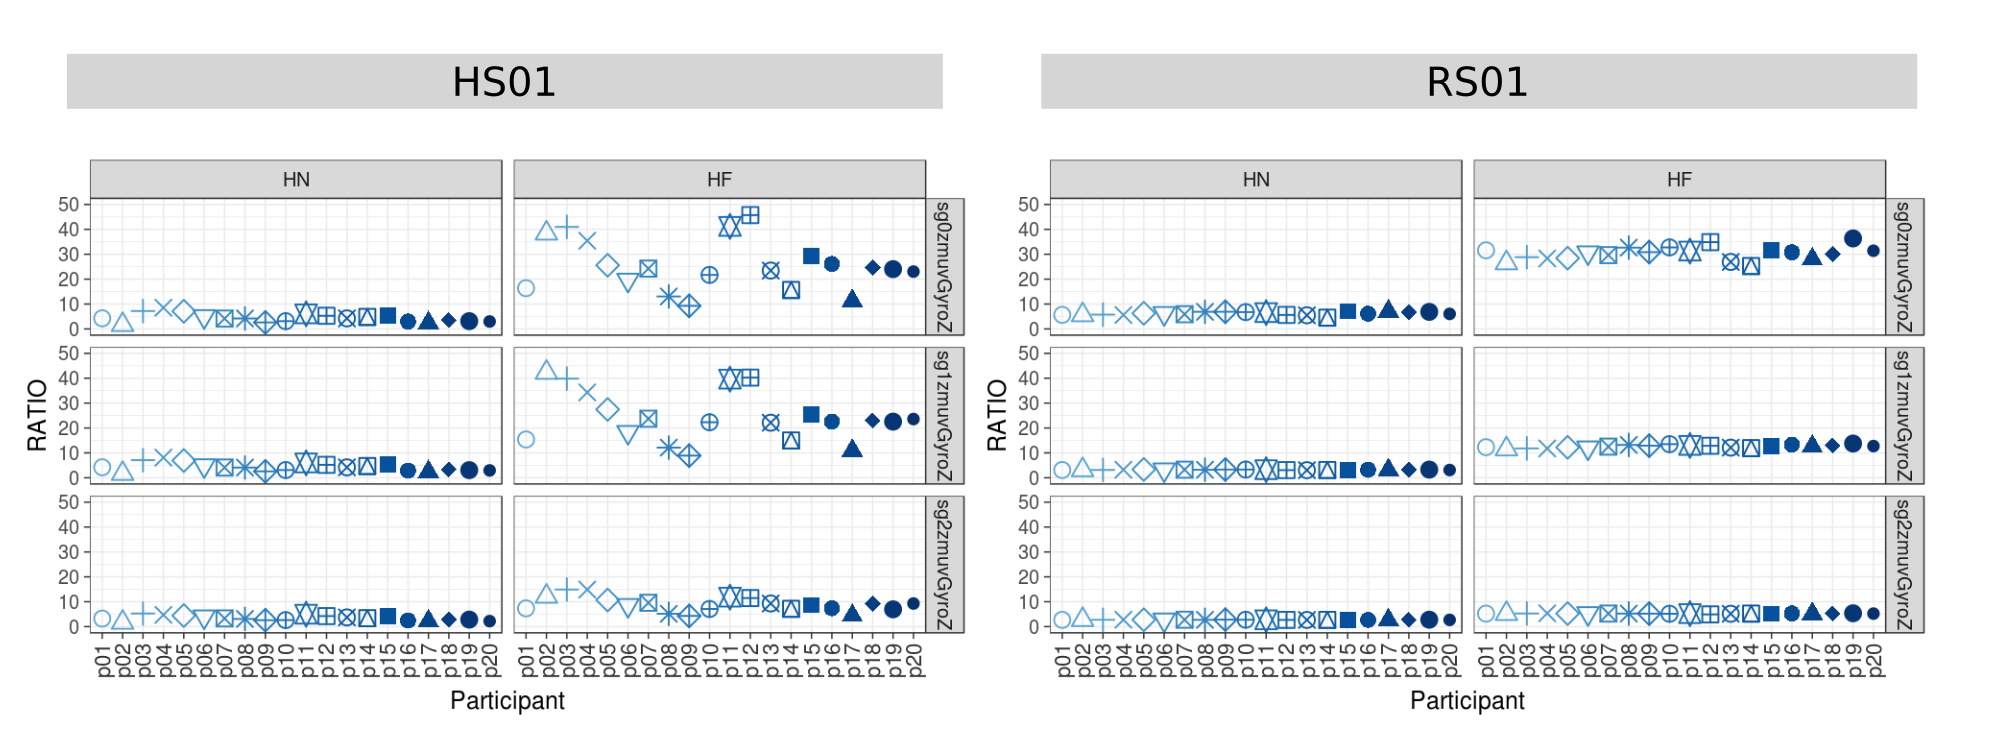
\includegraphics[width=1.0\textwidth]{ratio_aH}
    \caption{
	{\bf RATIO values for horizontal arm movements.}
	RATIO (representing dynamic transitions) for 
	20 participants performing HN and HF movements
	with sensors HS01, RS01 and three smoothed-normalised axis 
	of GyroZ (sg0zmuvGyroZ, sg1zmuvGyroZ and sg2zmuvGyroZ).
	RATIO values were computed with 
	embedding parameters $m=6$, $\tau=8$ and $\epsilon=1$.
	R code to reproduce the figure is available from \cite{hwum2018}.
        }
    \label{fig:ratio_aH}
\end{figure}
%%---------------------------------(FIGURE)------------------------------------
%%---------------------------------(FIGURE)-------------------------------------
\begin{figure}[!h]
\centering
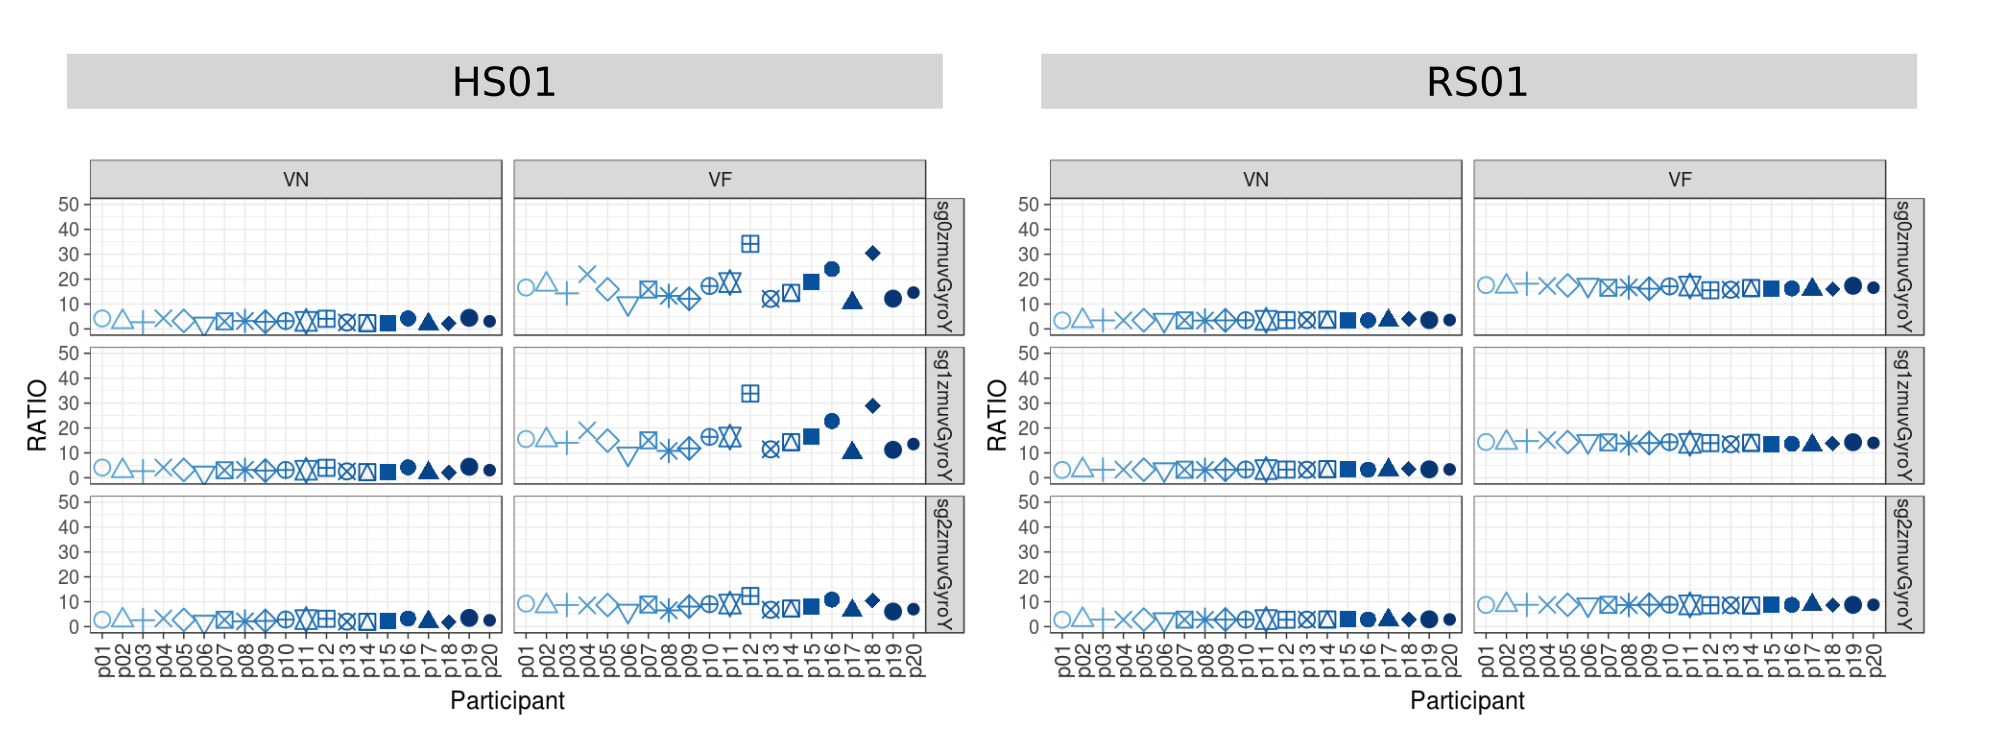
\includegraphics[width=1.0\textwidth]{ratio_aV}
    \caption{
	{\bf RATIO values for vertical arm movements.}
	RATIO (representing dynamic transitions) for 
	20 participants performing VN and VF movements
	with sensors HS01, RS01 and three smoothed-normalised axis 
	of GyroY (sg0zmuvGyroY, sg1zmuvGyroY and sg2zmuvGyroY).
	RATIO values were computed with
	embedding parameters $m=6$, $\tau=8$ and $\epsilon=1$.
	R code to reproduce the figure is available from \cite{hwum2018}.
        }
    \label{fig:ratio_aV}
\end{figure}
%%---------------------------------(FIGURE)------------------------------------


\subsubsection*{ENTR values}
ENTR values show more variation for HS01 sensor than ENTR values for RS01 sensor
which appear to be more constant and the smoothness of data affects little 
to the variation of ENTR values (Figs~\ref{fig:entr_aH} and \ref{fig:entr_aV}).
%%---------------------------------(FIGURE)-------------------------------------
\begin{figure}[!h]
\centering
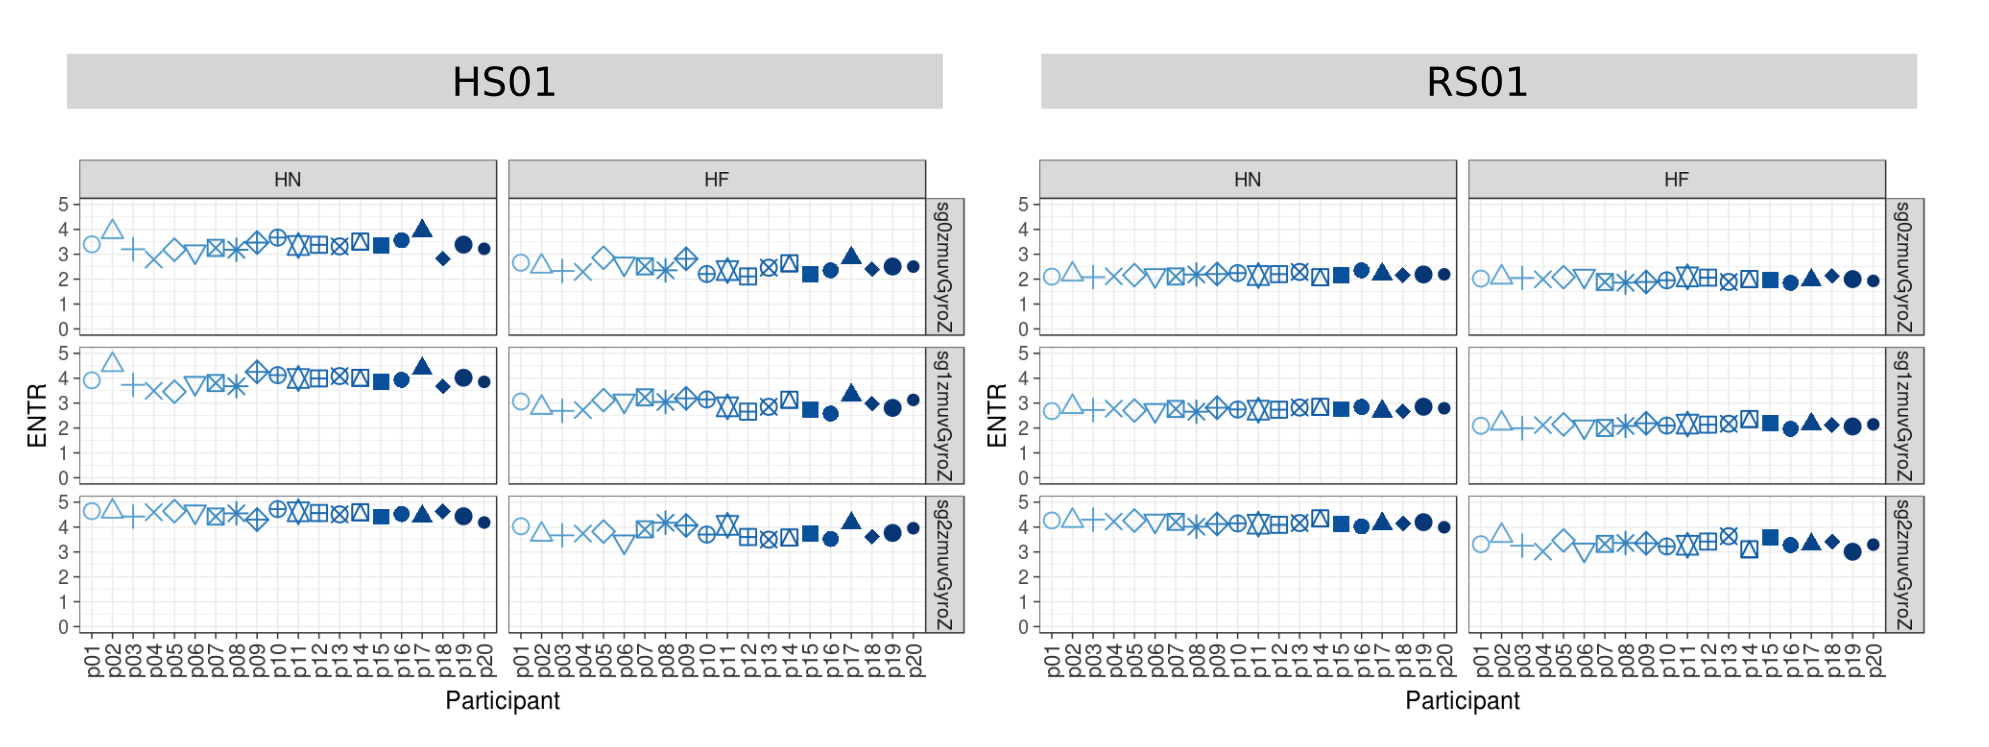
\includegraphics[width=1.0\textwidth]{entr_aH}
    \caption{
	{\bf ENTR values for horizontal arm movements.}
    	ENTR values (representing the complexity of the deterministic structure in time series) for 
	20 participants performing HN and HF movements
	with sensors HS01, RS01 and three smoothed-normalised axis 
	of GyroZ (sg0zmuvGyroZ, sg1zmuvGyroZ and sg2zmuvGyroZ).
	ENTR values were computed with 
	embedding parameters $m=6$, $\tau=8$ and $\epsilon=1$.
	R code to reproduce the figure is available from \cite{hwum2018}.
        }
    \label{fig:entr_aH}
\end{figure}
%%---------------------------------(FIGURE)------------------------------------
%%---------------------------------(FIGURE)-------------------------------------
\begin{figure}[!h]
\centering
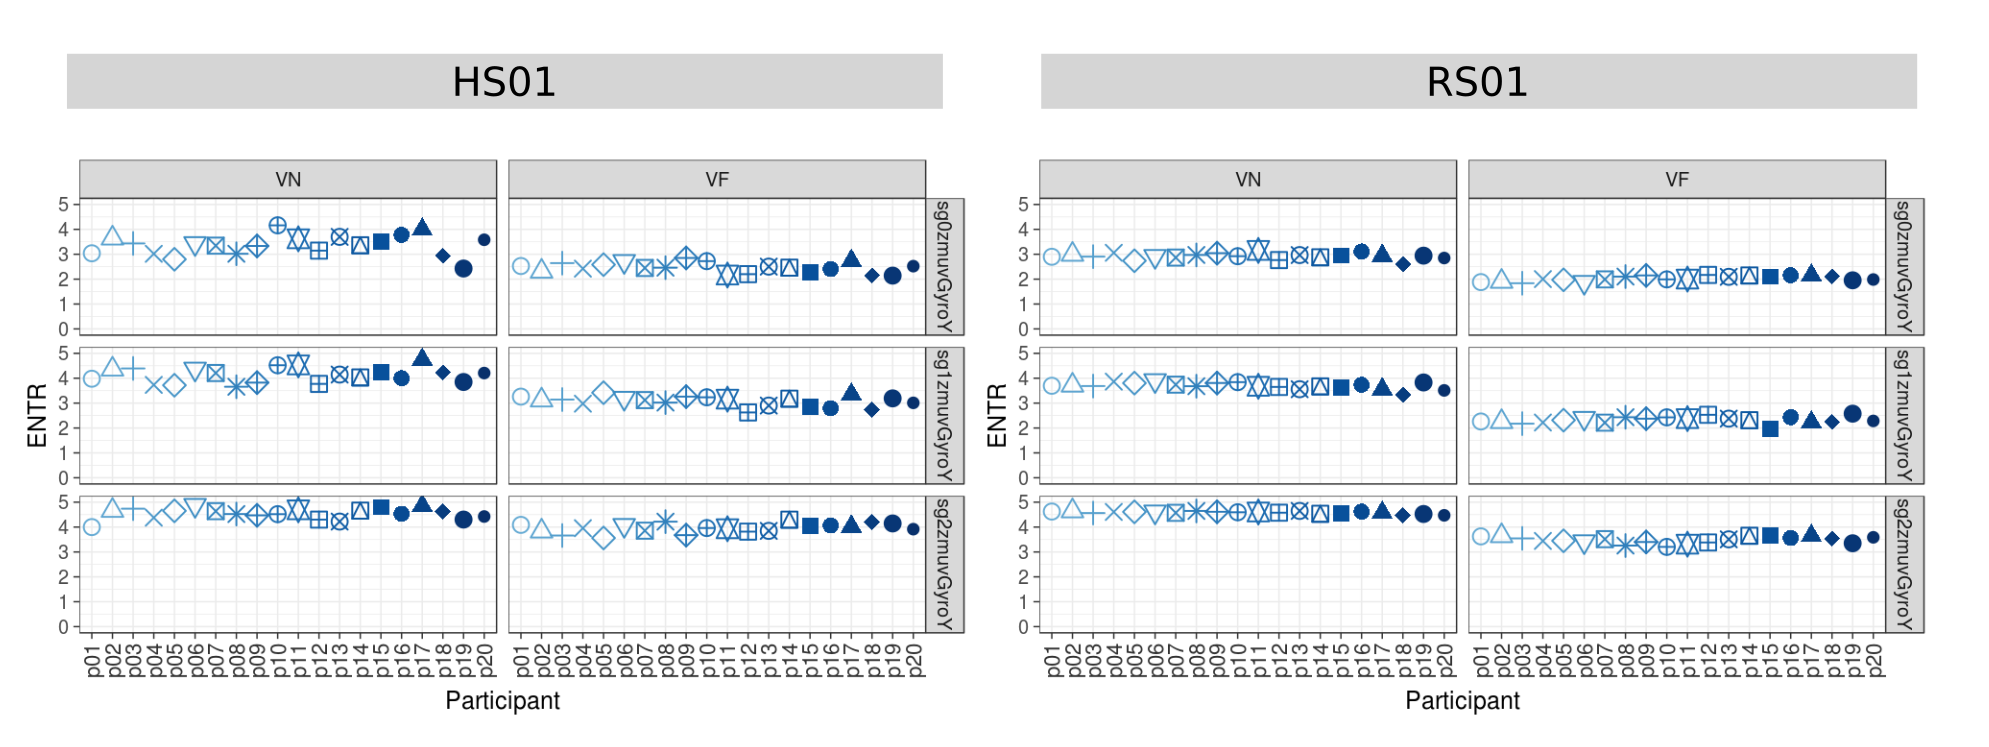
\includegraphics[width=1.0\textwidth]{entr_aV}
    \caption{
	{\bf ENTR values for vertical arm movements.}
    	ENTR values (representing the complexity of the deterministic structure in time series) for 
	20 participants performing VN and VF movements
	with sensors HS01, RS01 and three smoothed-normalised axis 
	of GyroY (sg0zmuvGyroY, sg1zmuvGyroY and sg2zmuvGyroY).
	ENTR values were computed with 
	embedding parameters $m=6$, $\tau=8$ and $\epsilon=1$.
	R code to reproduce the figure is available from \cite{hwum2018}.
        }
    \label{fig:entr_aV}
\end{figure}
%%---------------------------------(FIGURE)------------------------------------





%% \subsection{Effects of different parameters in the computation of different metrics of RQA.}
%Then we only select the axis AccY and GyroZ as being the axis which show 
%better consistency in the patters for all the posibilities int he time series.
%That was doing visual inspection. It also worthwhile to note that those axis
%represent the majoy energy amothn other axis for both sensors.
%The selection of recurrecne threshold is 1 for HF activites,
%however this should be changed to
%for HN activies.
%With that we also can observe the effect of the seletion 
%of recurrence threshold for different actibities is crucial 
%to have meaninign values in the metrics of RQA.
%% added: Tue 19 Jun 2018






\subsection{RQA metrics with different embedding parameters, recurrence thresholds, 
window lengths, levels of smoothness, and time series structures.}
Zbilut et al. \cite{zbilut1992} established RQA metrics with the aim of determining 
embedding parameters, their method consisted on creating 3D surfaces with RQA metrics 
with an increase of embedding parameters ($m$ and $\tau$), then 
Zbilut et al. \cite{zbilut1992} explored fluctuations and gradual changes in the 3D surfaces
that provide information about the embeddings.
Much recently, Marwan et al. \cite{marwan2015} created 3D surfaces for visual selection 
of not only embedding parameters but also recurrence thresholds. 
Following same methodologies, we explored the stability and robustness of RQA metrics (REC, DET, RATIO and ENTR)
using 3D surfaces by an unitary increase of the pair embedding parameters ($0 \ge m \le 10$, $0 \ge \tau \le 10$) 
and a decimal increase of 0.1 for recurrence thresholds ($ 0.2 \ge \epsilon \le 3 $) (Fig.~\ref{fig:topo_rqas}).
We also computed 3D surfaces of RQA metrics for different sensors and different activities (Fig.~\ref{fig:topo_sensoractivities}).
RQA metrics are also affected by the window length where for example four 
window lengths of 100, 250, 500 and 750 samples (Fig.~\ref{fig:topo_windows}).
Three level of smoothness were computed for RQA metrics showing 
smoothed 3D surfaces ad the level of smoothness increase (Fig.~\ref{fig:topo_smoothness}).
Similarly, 3D surfaces of RQA metrics were also computed for three participants (Fig.~\ref{fig:topo_participants}).
%%---------------------------------(FIGURE)-------------------------------------
\begin{figure}[!ht]
\centering
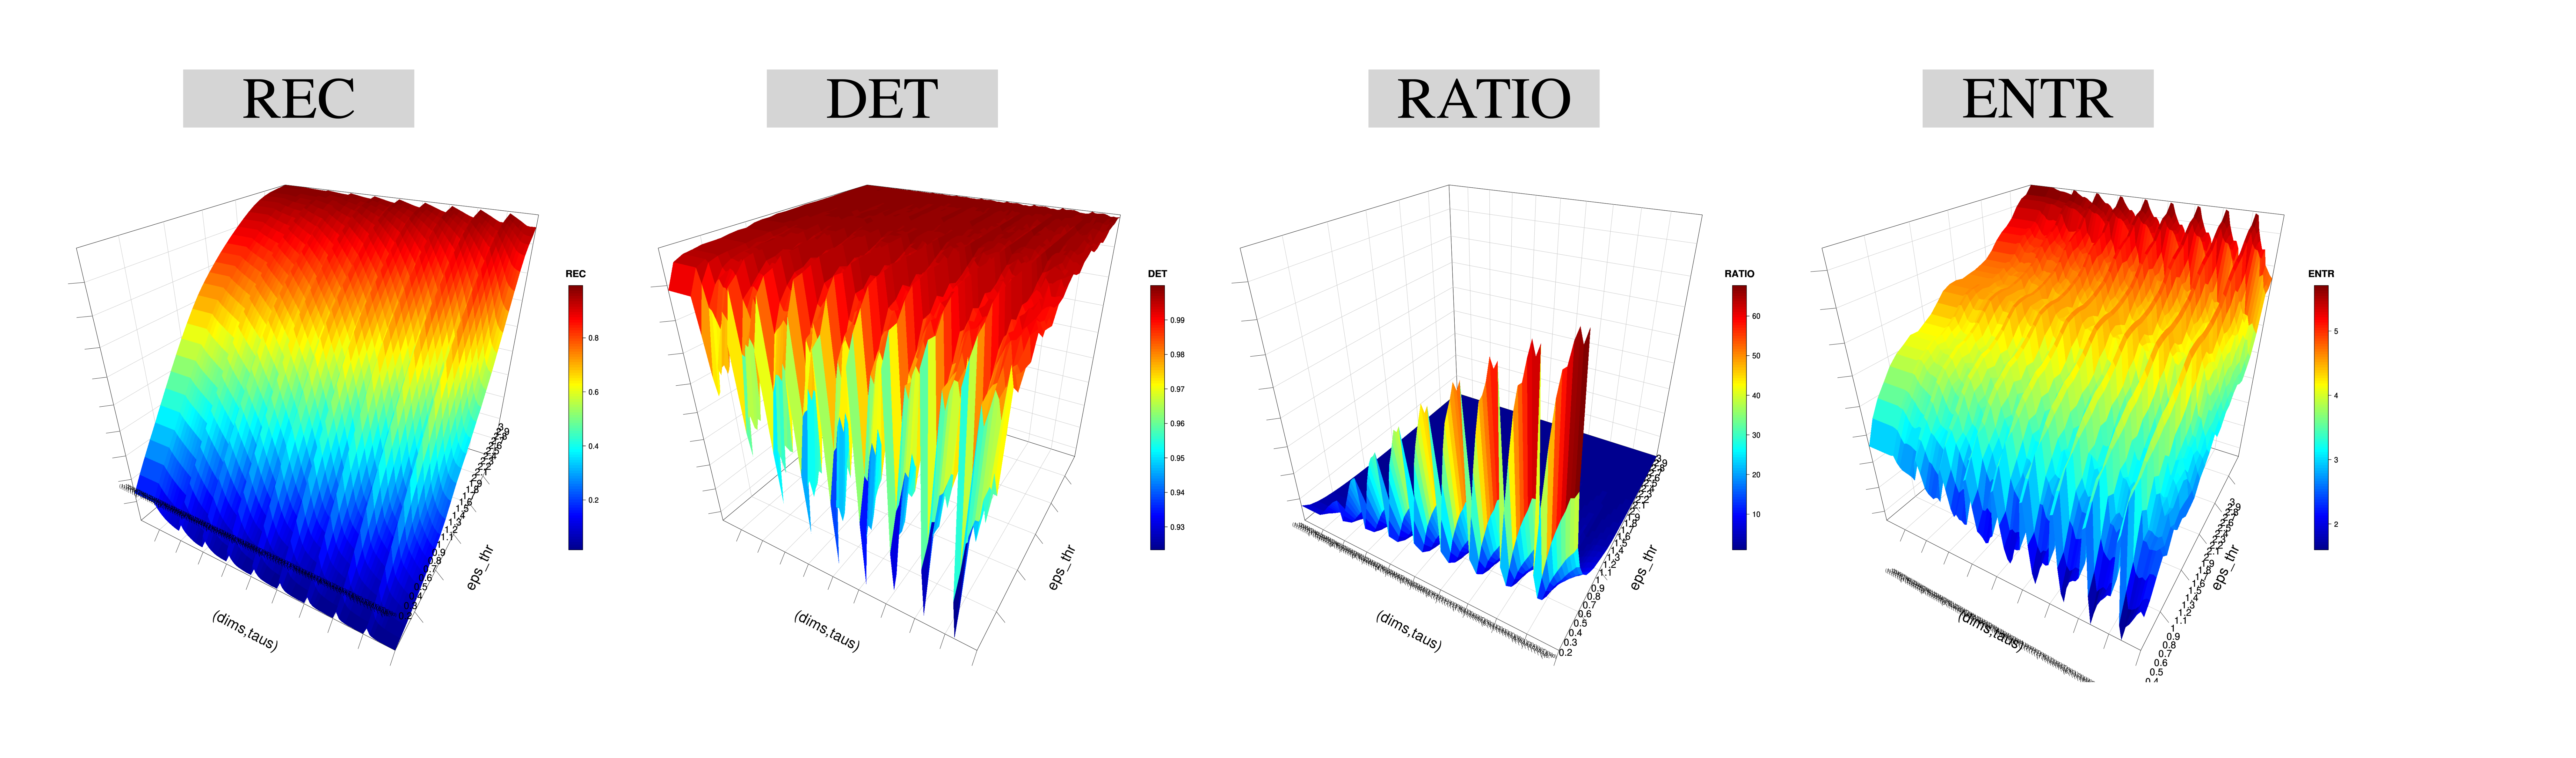
\includegraphics[width=1.0\textwidth]{rqas}
    \caption{
	{\bf 3D surfaces for RQA metrics.}
	3D surfaces for REC, DET, RATIO and ENTR values with increasing 
	pair embedding parameters ($0 \ge m \le 10$, $0 \ge \tau \le 10$) 
	and recurrence thresholds (  $ 0.2 \ge \epsilon \le 3 $).
	RQA metrics values for time series of participant p01 using HS01 sensor, 
	HN activity and sg0zmuvGyroZ axis and 500 samples window length.
        R code to reproduce the figure is available from \cite{hwum2018}.
	}
\label{fig:topo_rqas}
\end{figure}
%%---------------------------------(FIGURE)------------------------------------
%%---------------------------------(FIGURE)-------------------------------------
\begin{figure}[!ht]
\centering
\includegraphics[width=1.0\textwidth]{sa}
    \caption{
	{\bf 3D surfaces of RQA metrics for sensors and activities.}
	3D surfaces with increasing embedding parameters and recurrence thresholds are 
	for HS01 and RS01 sensors of HN, HF, VN and VF activities.
	RQA metrics values are for time series of participant p01 for sensors (HS01 and RS01), 
	activities (HN, HF, VN and VF) and for 	sg0zmuvGyroZ axis  with 500 samples window length. 
	R code to reproduce the figure is available from \cite{hwum2018}.
       }
\label{fig:topo_sensoractivities}
\end{figure}
%%---------------------------------(FIGURE)-------------------------------------
%%---------------------------------(FIGURE)-------------------------------------
\begin{figure}[!ht]
\centering
\includegraphics[width=1.0\textwidth]{w}
    \caption{
	{\bf 3D surfaces for RQAs metrics with four window lengths.}
	3D surfaces of RQAs metric values with increasing embedding parameters and recurrence thresholds 
	are for four window lengths (w100, w250, w500 and  w750).
	RQA metrics values are for time series of participant p01 
	using HS01 sensor, HN activity and sg0zmuvGyroZ axis.
	R code to reproduce the figure is available from \cite{hwum2018}.
        }
\label{fig:topo_windows}
\end{figure}
%%---------------------------------(FIGURE)------------------------------------
%%---------------------------------(FIGURE)-------------------------------------
\begin{figure}[!ht]
\centering
\includegraphics[width=1.0\textwidth]{s}
    \caption{
	{\bf 3D surfaces for RQA metrics with three levels of smoothness.}
       	3D surfaces of RQAs metric values with increasing embedding parameters and recurrence thresholds 
	are for three levels of smoothness (sg0zmuvGyroZ, sg1zmuvGyroZ and sg1zmuvGyroZ).
	RQA metrics values are for time series of participant p01 using HS01 sensor, 
	HN activity and 500 samples window length.
	R code to reproduce the figure is available from \cite{hwum2018}.
 }
\label{fig:topo_smoothness}
\end{figure}
%%---------------------------------(FIGURE)------------------------------------


%%---------------------------------(FIGURE)-------------------------------------
\begin{figure}[!ht]
\centering
\includegraphics[width=1.0\textwidth]{p}
    \caption{
	{\bf 3D surfaces for RQA metrics with three participants.}
       	3D surfaces of RQAs metric values for participants p01, p02 and p03 
	with increasing embedding parameters and recurrence thresholds.
	RQA metrics values are for time series of HS01 sensor, 
	HN activity and 500 samples window length.
	R code to reproduce the figure is available from \cite{hwum2018}.
 }
\label{fig:topo_participants}
\end{figure}
%%---------------------------------(FIGURE)------------------------------------








